\documentclass{classrep}
\usepackage[utf8]{inputenc}


\studycycle{Informatyka, studia dzienne, inż I st.}
\coursesemester{V}
\coursename{Obliczenia naukowe}
\courseyear{2017/2018}
\courseteacher{dr hab. Paweł Zieliński}
\coursegroup{czwartek TN, 11:15}

\author{
  \studentinfo{Agata Jasionowska}{229726}
}

\title{Laboratorium \ppauza Lista 4}
\begin{document}

\maketitle

\section{Zadanie 1}
	\subsection{Opis problemu}
		Zadanie polegało na implementacji funkcji obliczającej ilorazy różnicowe na podstawie podanego wektora węzłów oraz wartości funkcji, jednak bez użycia tablicy dwuwymiarowej.
		
		Iloraz różnicowy $k$-tego rzędu spełnia poniższą zależność:
		$$f[x_0,x_1, \ldots, x_k] = \frac{f[x_1,x_2, \ldots, x_k] - f[x_0, x_1, \ldots, x_{k-1}]}{x_k - x_0},$$
		zaś ilorazy rzędu zerowego oraz pierwszego równe są kolejno:
		$$f[x_0] = f(x_0), \qquad f[x_0,x_1] = \frac{f(x_1) - f(x_0)}{x_1 - x_0}.$$
		
	
	\subsection{Opis rozwiązania}
		Znając węzły $x_k$ i wartości funkcji $f(x_k)$ (czyli również ilorazy $f[x_k]$ zerowego rzędu) można za pomocą tego wzoru utworzyć dwuwymiarową tablicę ilorazów różnicowych wyższych rzędów. Jednak algorytm takiej konstrukcji jest nieefektywny, gdyż wystarczy użyć jednowymiarowej tablicy $d$ zmiennych z jednym wskaźnikiem. Początkowymi wartościami zmiennych $d_i$ są odpowiadające im $f[x_i]$, czyli każde $d_i$ obliczane jest ze wzoru:
		$$d_i = \frac{d_i-d_{i-1}}{x_i-x_{i-j}}, $$	
		gdzie $j$ oznacza numer kolumny.	
		Każda kolejna wartość uaktualniana jest kolumnami, zaś wewnątrz każdej kolumny - z dołu do góry. Dzięki takiej kolejności obliczeń tablica $d$ zawiera w każdej chwili ilorazy, które będą później potrzebne. 
		
		Szczegółowy przebieg metody został przedstawiony w Algorytmie \ref{algo:1}.
		
		\begin{algorithm}[!h]
			\SetKwInOut{Input}{Input}
    			\SetKwInOut{Output}{Output}
    			\SetKw{KwDownTo}{downto}
    			\SetKwProg{Fun}{Function}{}{}
    			\SetKwFunction{iloraz}{ilorazyRoznicowe}
			\SetKwData{X}{x}
			\SetKwData{F}{f}
			\SetKwData{Fx}{fx}
			\SetKwData{I}{i}
			\SetKwData{J}{j}
			\SetKwData{N}{n}
			
			\Input{
					\begin{tabular}{rcl}
    						{\X} &---& wektor długości $n+1$ zawierający węzły $x_0, \ldots, x_n$,\\
    						{\F} &---& wektor długości $n+1$ zawierający wartości interpolowanej funkcji\\
    								&& w węzłach $f(x_0), \ldots, f(x_n)$.
					\end{tabular}
		    			}
		    \Output{
		    			\begin{tabular}{rcl}
			    			{\Fx} & {---} & wektor długości $n+1$ zawierający obliczone ilorazy różnicowe. 			
					\end{tabular}
		    	}
		    	
    			\Fun{\iloraz{\X, \F}} {
    				\For{\I $\gets 1$ \KwTo \N} {
		    			$\Fx[\I]\gets\F[\I]$\;
		    		}
		    		\For{\J $\gets 1$ \KwTo \N} {
			    		\For{\I $\gets$\N \KwDownTo \I} {
			    			$\Fx[\I] \gets (\Fx[\I] - \Fx[\I - 1]) / (\X[\I] - \X[\I - \J])$\;
		    			}
		    		}
				\KwRet \Fx\;
		    }
    			\caption{Ilorazy różnicowe}
    			\label{algo:1}
		\end{algorithm}		
	
\section{Zadanie 2}
	\subsection{Opis problemu}
		Zadanie polegało na implementacji funkcji obliczającej wartość wielomianu interpolacyjnego stopnia $n$ w postaci Newtona $N_n(x)$ w zadanym punkcie za pomocą uogólnionego algorytmu Hornera.
		$$N_n(x) = \sum_{i=0}^k c_i \prod_{j=0}^{i-1}(x-x_j),$$
		gdzie $c_i$ jest ilorazem różnicowym stopnia $i$, zaś $x_j$ --- węzłem interpolacji.
		
		Metoda Newtona, pomimo iż jest trudniejsza w implementacji niż np metoda Lagrange'a i wymaga większej ilości oddzielnych "kroków", jest dużo lepiej uwarunkowana numerycznie, przez co warta poznania pod kątem stosowania na maszynach cyfrowych. W metodzie najpierw wyznaczane są odpowiednie ilorazy różnicowe, a dopiero później z ich użyciem --- interpolowana funkcja.
				
	\subsection{Opis rozwiązania}	
		W rozwiązaniu zadania posłużono się uogólnionym algorytmem Hornera, który prezentuje się następująco:
		$$\begin{aligned}
			&w_n(x) := f[x_0, x_1, \ldots, x_n];&\\
			&w_k(x) := w_{k+1}(x-x_k)+ f[x_0, x_1, \ldots, x_k]	\quad(k=n-1, n-2, \ldots, 0);&\\
			&N_n(x) = w_0(x).
		\end{aligned}$$
		
		Na jego podstawie możliwe było napisanie funkcji wyznaczającej wartość wielomianu w punkcie w czasie O(n).
		Szczegóły przedstawiono poniżej (Algorytm \ref{algo:2}).
	
		\begin{algorithm}[!htbp]
			\SetKwInOut{Input}{Input}
    			\SetKwInOut{Output}{Output}
    			\SetKw{KwDownTo}{downto}
    			\SetKwProg{Fun}{Function}{}{}
    			\SetKwFunction{LEN}{length}
    			\SetKwFunction{F}{warNewton}
			\SetKwData{X}{x}
			\SetKwData{FX}{fx}
			\SetKwData{T}{t}
			\SetKwData{NT}{nt}
			\SetKwData{N}{n}
			\SetKwData{I}{i}

			\Input{
					\begin{tabular}{rcl}
    						{\X} &---& wektor długości $n+1$ zawierający węzły $x_0, \ldots, x_n$,\\
    						{\FX} &---& wektor długości $n+1$ zawierający ilorazy różnicowe,\\
    						{\T} &---& punkt, w którym należy obliczyć wartość wielomianu.
					\end{tabular}
		    			}
		    \Output{	
		    			\begin{tabular}{rcl}
			    			{\NT} & {---} & wartość wielomianu w punkcie \T.
					\end{tabular}
		    	}
		    	
    			\Fun{\F{\X, \FX, \T}} {
		    		\N $\gets$ \LEN{\FX}\;
		    		\NT $\gets \FX[\N]$\;
		    		\For{\I $\gets \N-1$ \KwDownTo $1$} {
		    			\NT $\gets \FX[\I] + (\T - \X[\I]) * \NT$\; 		
		    		}
		    		\KwRet \NT\;
    			}
    			\caption{Wielomian interpolacyjny Newtona.}
    			\label{algo:2}
		\end{algorithm}	

\section{Zadanie 3}
	\subsection{Opis problemu}
		Zadanie polegało na implementacji funkcji obliczającej współczynniki postaci naturalnej wielomianu interpolacyjnego w postaci Newtona.
				
	\subsection{Opis rozwiązania}
		U podstaw rozwiązania problemu wyznaczenia współczynników naturalnych leży stosunkowo prosty mechanizm. Otóż w wielomianie interpolacyjnym współczynnik $a_n$ przy najwyższej potędze argumentu jest równe $c_n$, zaś z tego faktu, posługując się wspomnianym już wcześniej uogólnionym algorytmem Hornera, wynika także, że $w_n$ jest również równy $a_n$. Bazując na uzyskanej równości każdy kolejny krok algorytmu będzie polegał na tworzeniu wartości $a_i$ w oparciu o współczynniki uprzednio policzone (stojące przy wyższych potęgach). 
		Znalezienie zależności pomiędzy kolejnymi $a_i$ polega na przejściu po wszystkich $w_i$ w dół (poczynając od $i = n$) i modyfikowaniu współczynników tak, aby dla każdego $w_i$ doprowadzić w danym momencie do postaci naturalnej. Nietrudno wyliczyć zmiany wprowadzane w każdym $a_i$, zatem uzyskanie takiej postaci przy każdym przebiegu nie nastręcza problemów. 
		
		Działanie tej metody prezentuje Algorytm \ref{algo:3}.
	
		\begin{algorithm}[!htbp]
			\SetKwInOut{Input}{Input}
    			\SetKwInOut{Output}{Output}
    			\SetKw{KwDownTo}{downto}
    			\SetKwProg{Fun}{Function}{}{}
    			\SetKwFunction{LEN}{length}
    			\SetKwFunction{F}{naturalna}
			\SetKwData{X}{x}
			\SetKwData{FX}{fx}
			\SetKwData{A}{a}
			\SetKwData{J}{k}
			\SetKwData{I}{i}
			\SetKwData{N}{m}
			\SetKwData{P}{p}
			
			\Input{
					\begin{tabular}{rcl}
    						{\X} &---& wektor długości $n+1$ zawierający węzły $x_0, \ldots, x_n$,\\
    						{\FX} &---& wektor długości $n+1$ zawierający ilorazy różnicowe.
					\end{tabular}
		    			}
		    \Output{	
		    			\begin{tabular}{rcl}
			    			{\A} & {---} & wektor długości $n+1$ zawierający obliczone współczynniki postaci \\
			    				&& naturalnej.
					\end{tabular}
		    	}

		    	\Fun{\F{\X, \FX}} {
		    		\N $\gets$ \LEN{\FX}\;
		    		\A[\N] $\gets \FX[\N]$\;
		    		\For{\I $\gets \N-1$ \KwDownTo $1$} {
		    			\P $\gets \A[\I+1] * \X[\I]$\;
		    			$\A[\I] \gets \FX[\I] - \P$\; 
		    			\For{$\J \gets \I+1$ \KwTo $\N-1$} {
		    				\P $\gets \A[\J+1] * \X[\I]$\;
		    				$\A[\J] \gets \A[\J] - \P$\; 	
					}	
		    		}
		    		\KwRet \A\;
    			}

    			\caption{Współczynniki naturalne wielomianu interpolacyjnego.}
    			\label{algo:3}
		\end{algorithm}	
				
\section{Zadanie 4}
	\subsection{Opis problemu}
		Zadanie polegało na implementacji funkcji, która interpoluje zadaną funkcję $f(x)$ w przedziale $[a,b]$ za pomocą wielomianu interpolacyjnego stopnia $n$ w postaci Newtona, a następnie rysuje ten wielomian oraz $f(x)$.

	\subsection{Opis rozwiązania}
		Funkcja \texttt{rysujNnfx} rozpoczyna od wyznaczenia węzłów interpolacji oraz wartości, jakie przyjmuje w nich funkcja $f$, a następnie oblicza ilorazy różnicowe (\texttt{ilorazyRoznicowe} z Zadania 1.) dla zadanych węzłów. W celu uzyskania bardziej precyzyjnych wykresów, funkcję jak i wielomian interpolacyjny poddano próbkowaniu --- $25\cdot (n+1)$ równooddalonych punktów, dla których to obliczane są wartości wielomianu z wykorzystaniem funkcji \texttt{warNewton} z Zadania 2. Wygenerowane w ten sposób dane służą narysowaniu finalnych wykresów, które zrealizowano przy pomocy funkcji pakietu \texttt{Gadfly}.
		
		Przebieg tej metody następuje zgodnie z Algorytmem \ref{algo:4}.
		
		\begin{algorithm}[!htbp]
			\SetKwInOut{Input}{Input}
    			\SetKwInOut{Output}{Output}
    			\SetKw{KwDownTo}{downto}
    			\SetKwProg{Fun}{Function}{}{}
    			
    			\SetKwFunction{LEN}{length}
    			\SetKwFunction{Ff}{rysujNnfx}
    			\SetKwFunction{iloraz}{ilorazyRoznicowe}{}
    			\SetKwFunction{NEW}{warNewton}{}
    			\SetKwFunction{DRAW}{rysuj}{}
    			
			\SetKwData{F}{f}
			\SetKwData{FX}{fx}
			\SetKwData{A}{a}
			\SetKwData{B}{b}
			\SetKwData{N}{n}
			\SetKwData{KH}{kh}
			\SetKwData{MAX}{max}
			\SetKwData{H}{h}
			\SetKwData{I}{i}
			\SetKwData{X}{x}
			\SetKwData{Y}{y}
			\SetKwData{MULT}{mult}
			\SetKwData{PLX}{plot\_x}
			\SetKwData{PLY}{plot\_y}
			\SetKwData{PLH}{plot\_h}

			\Input{
					\begin{tabular}{rcl}
    						{\F} &---& funkcja $f(x)$ zadane jako anonimowa funkcja,\\
    						{\A,\B} &---& przedział interpolacji,\\
    						{\N} &---& stopień wielomiany interpolacyjnego.
					\end{tabular}
		    			}
		    \Output{	
		    			\begin{tabular}{rcl}
			    			{\quad} & {---} & Funkcja rysuje wielomian interpolacyjny i interpolowaną funkcję\\
			    			&& w przedziale $[\A,\B]$.
					\end{tabular}
		    	}

		    	
    			\Fun{\Ff{\F, \A, \B, \N}} {
		    		\KH $\gets$ 0\;
		    		\MAX $\gets \N+1$\;
		    		\H $\gets (\B-\A)/(\MAX-1)$\;
		    		\MULT $\gets 25$\;
		    		\For{\I $\gets 1$ \KwTo \MAX} {
		    			$\X[\I] \gets \A + \KH$\;
		    			$\Y[\I] \gets \F(\X[\I])$\;	
		    			\KH $\gets$ \KH + \H\;
		    		}
		    		\FX $\gets$ \iloraz{\X, \Y}\;
		    		\KH $\gets 0$\;
		    		\MAX $\gets$ \MAX * \MULT\;
		    		\H $\gets (\B-\A)/(\MAX-1)$\;
		    		\For{\I $\gets 1$ \KwTo \MAX} {
		    			$\PLX[\I] \gets \A + \KH$\;
		    			$\PLH[\I] \gets$ \NEW{\X, \FX, $\PLX[\I]$}\;
		    			$\PLY[\I] \gets \F(\PLX[\I])$\;	
		    			\KH $\gets$ \KH + \H\;
		    		}
		    		\DRAW{\PLX, \PLY}\;
		    		\DRAW{\PLX, \PLH}\;
    			}
   			\caption{Rysowanie funkcji oraz wielomianu ją interpolującego.}
    			\label{algo:4}
		\end{algorithm}	
		
\section{Zadanie 5}	
	\subsection{Opis problemu}
		Celem zadania było przetestowanie utworzonej w Zadaniu 4. funkcji \texttt{rysujNnfx} na następujących przykładach:
			\begin{enumerate}[(a)]
				\item $\exp{x},~ [0,1],~ n = 5, 10, 15$,
				\item $x^2 \sin{x},~ [-1,1],~ n = 5, 10, 15$.
			\end{enumerate}
	\subsection{Opis rozwiązania}	
		Funkcję \texttt{rysujNnfx} wywołano dla powyższych danych.
		
	\subsection{Wyniki}
		Uzyskane wykresy przedstawiono na Rysunkach \ref{fig:1}-\ref{fig:2}.
			
		\begin{figure}[!h]
			\centering
			\subfloat[1.][$n=5$]{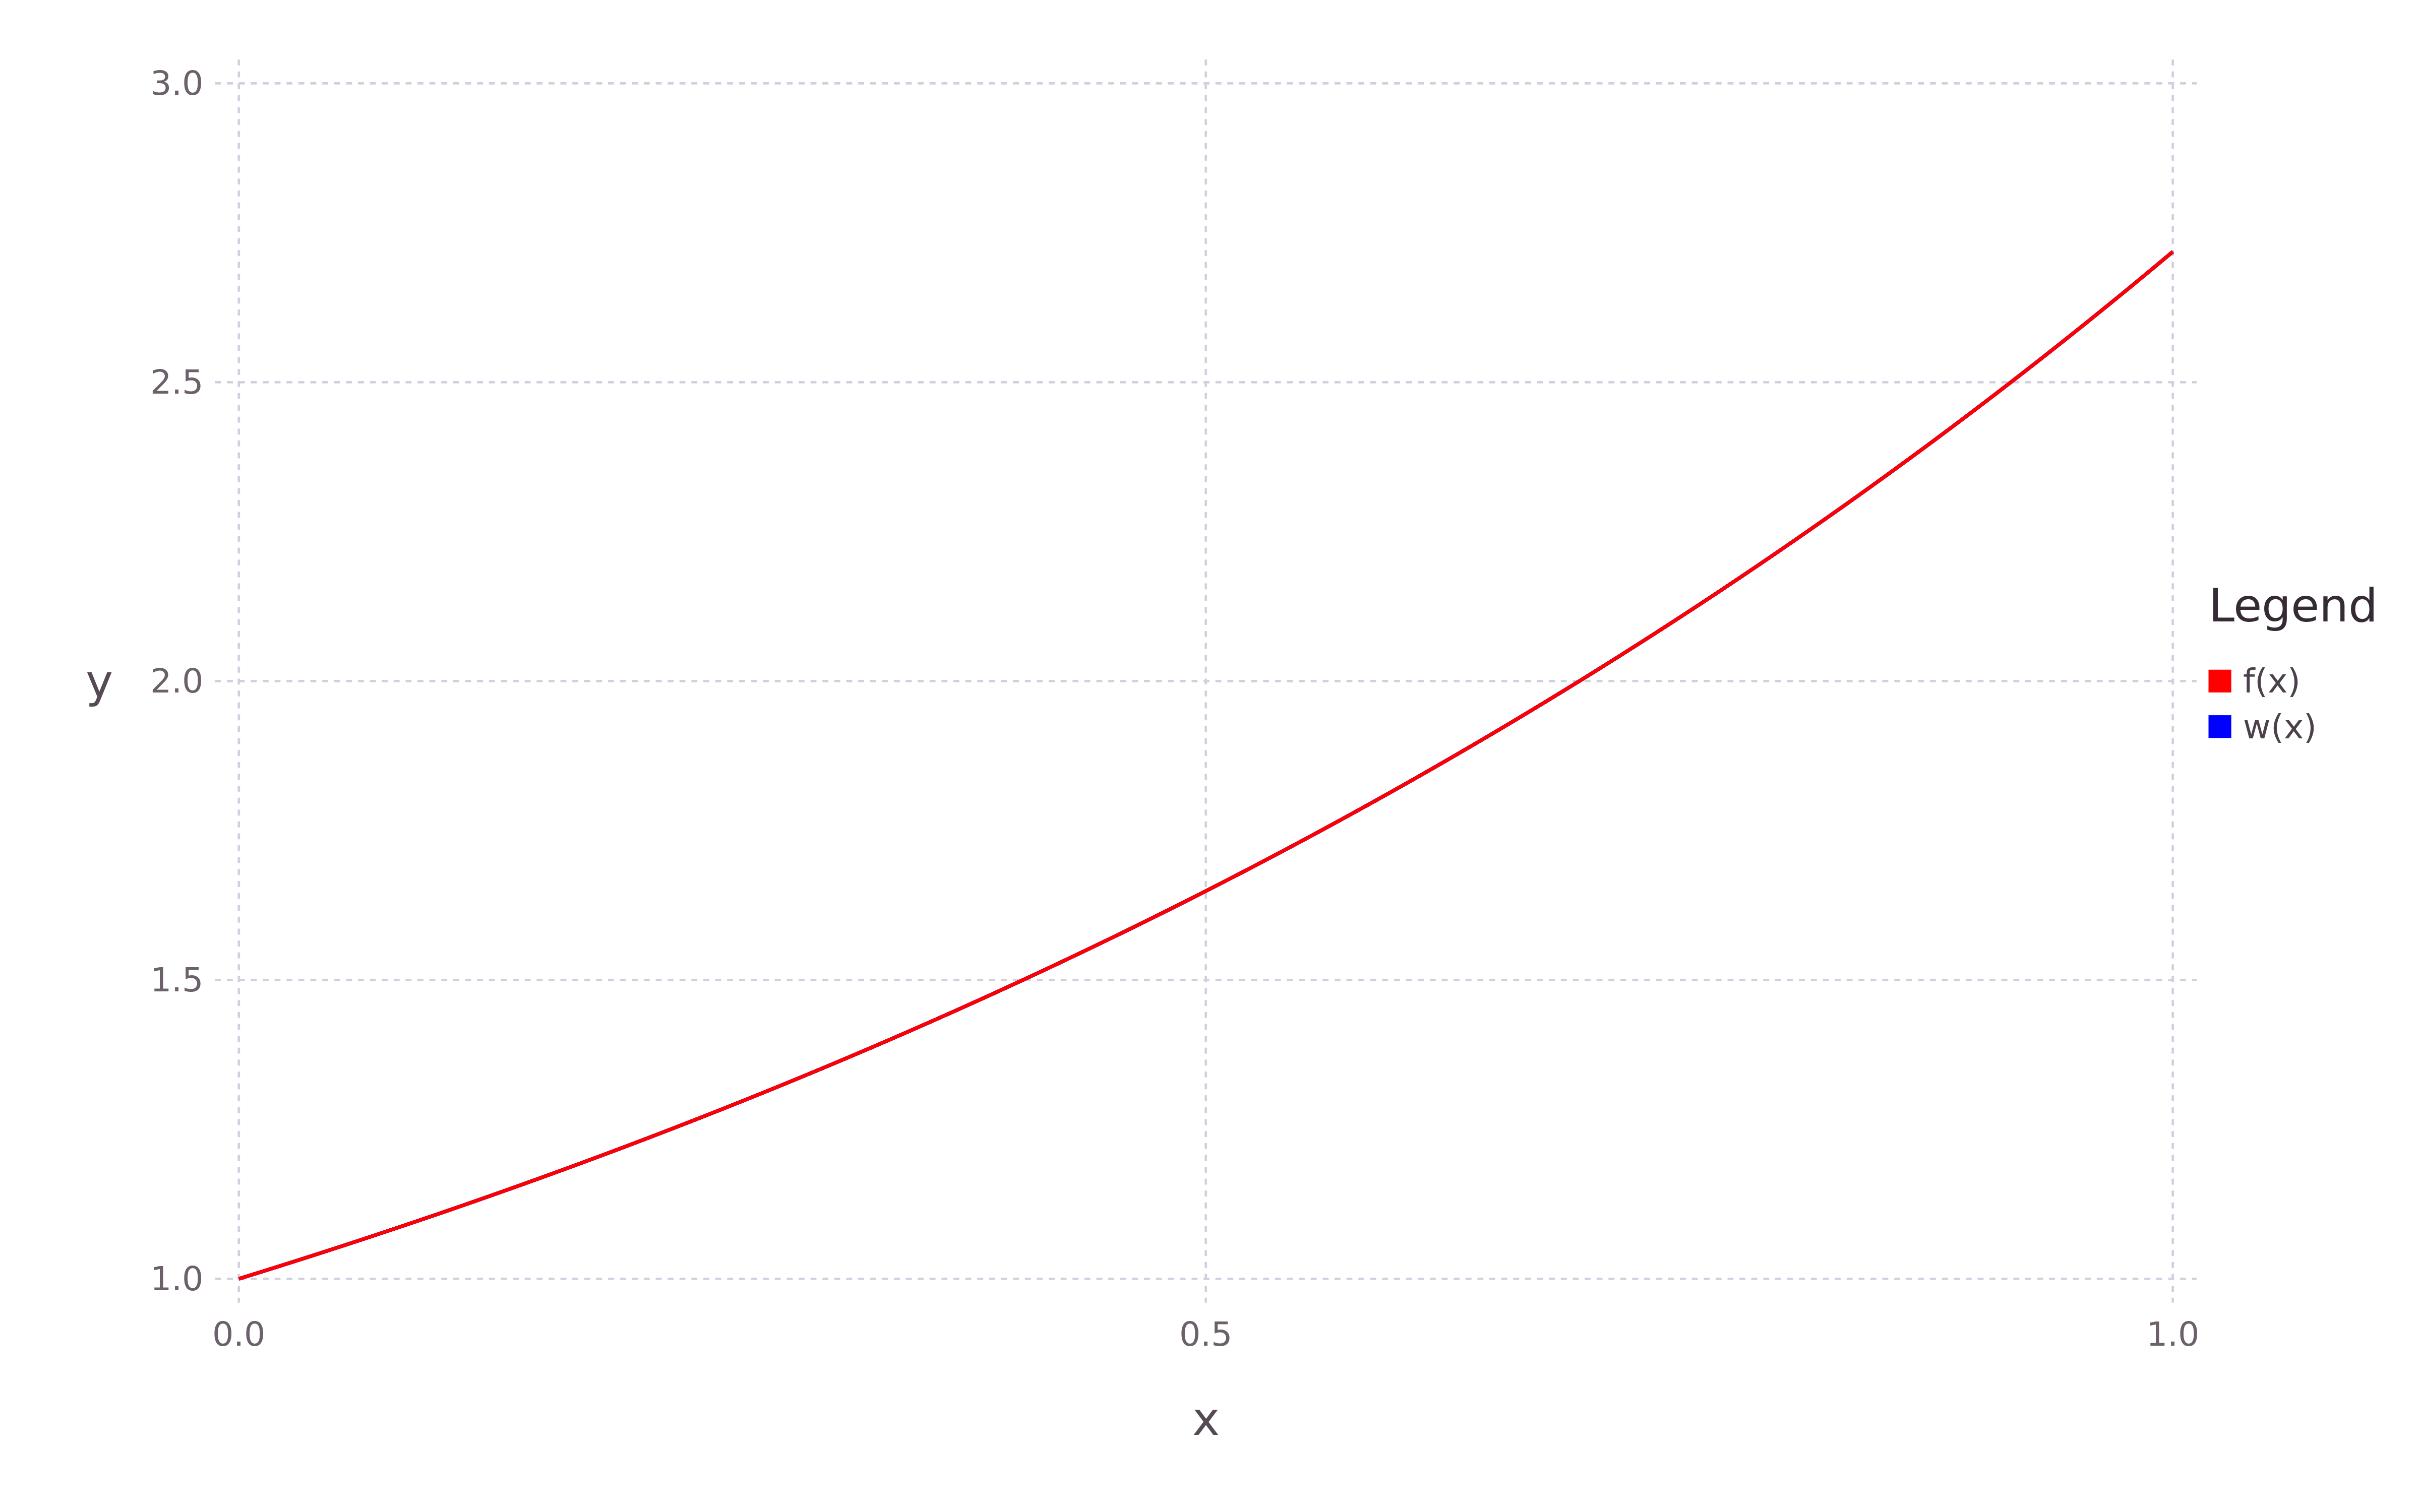
\includegraphics[width=0.5\textwidth]{zad5/plota1.png}} \hfill
			\subfloat[2.][$n=10$]{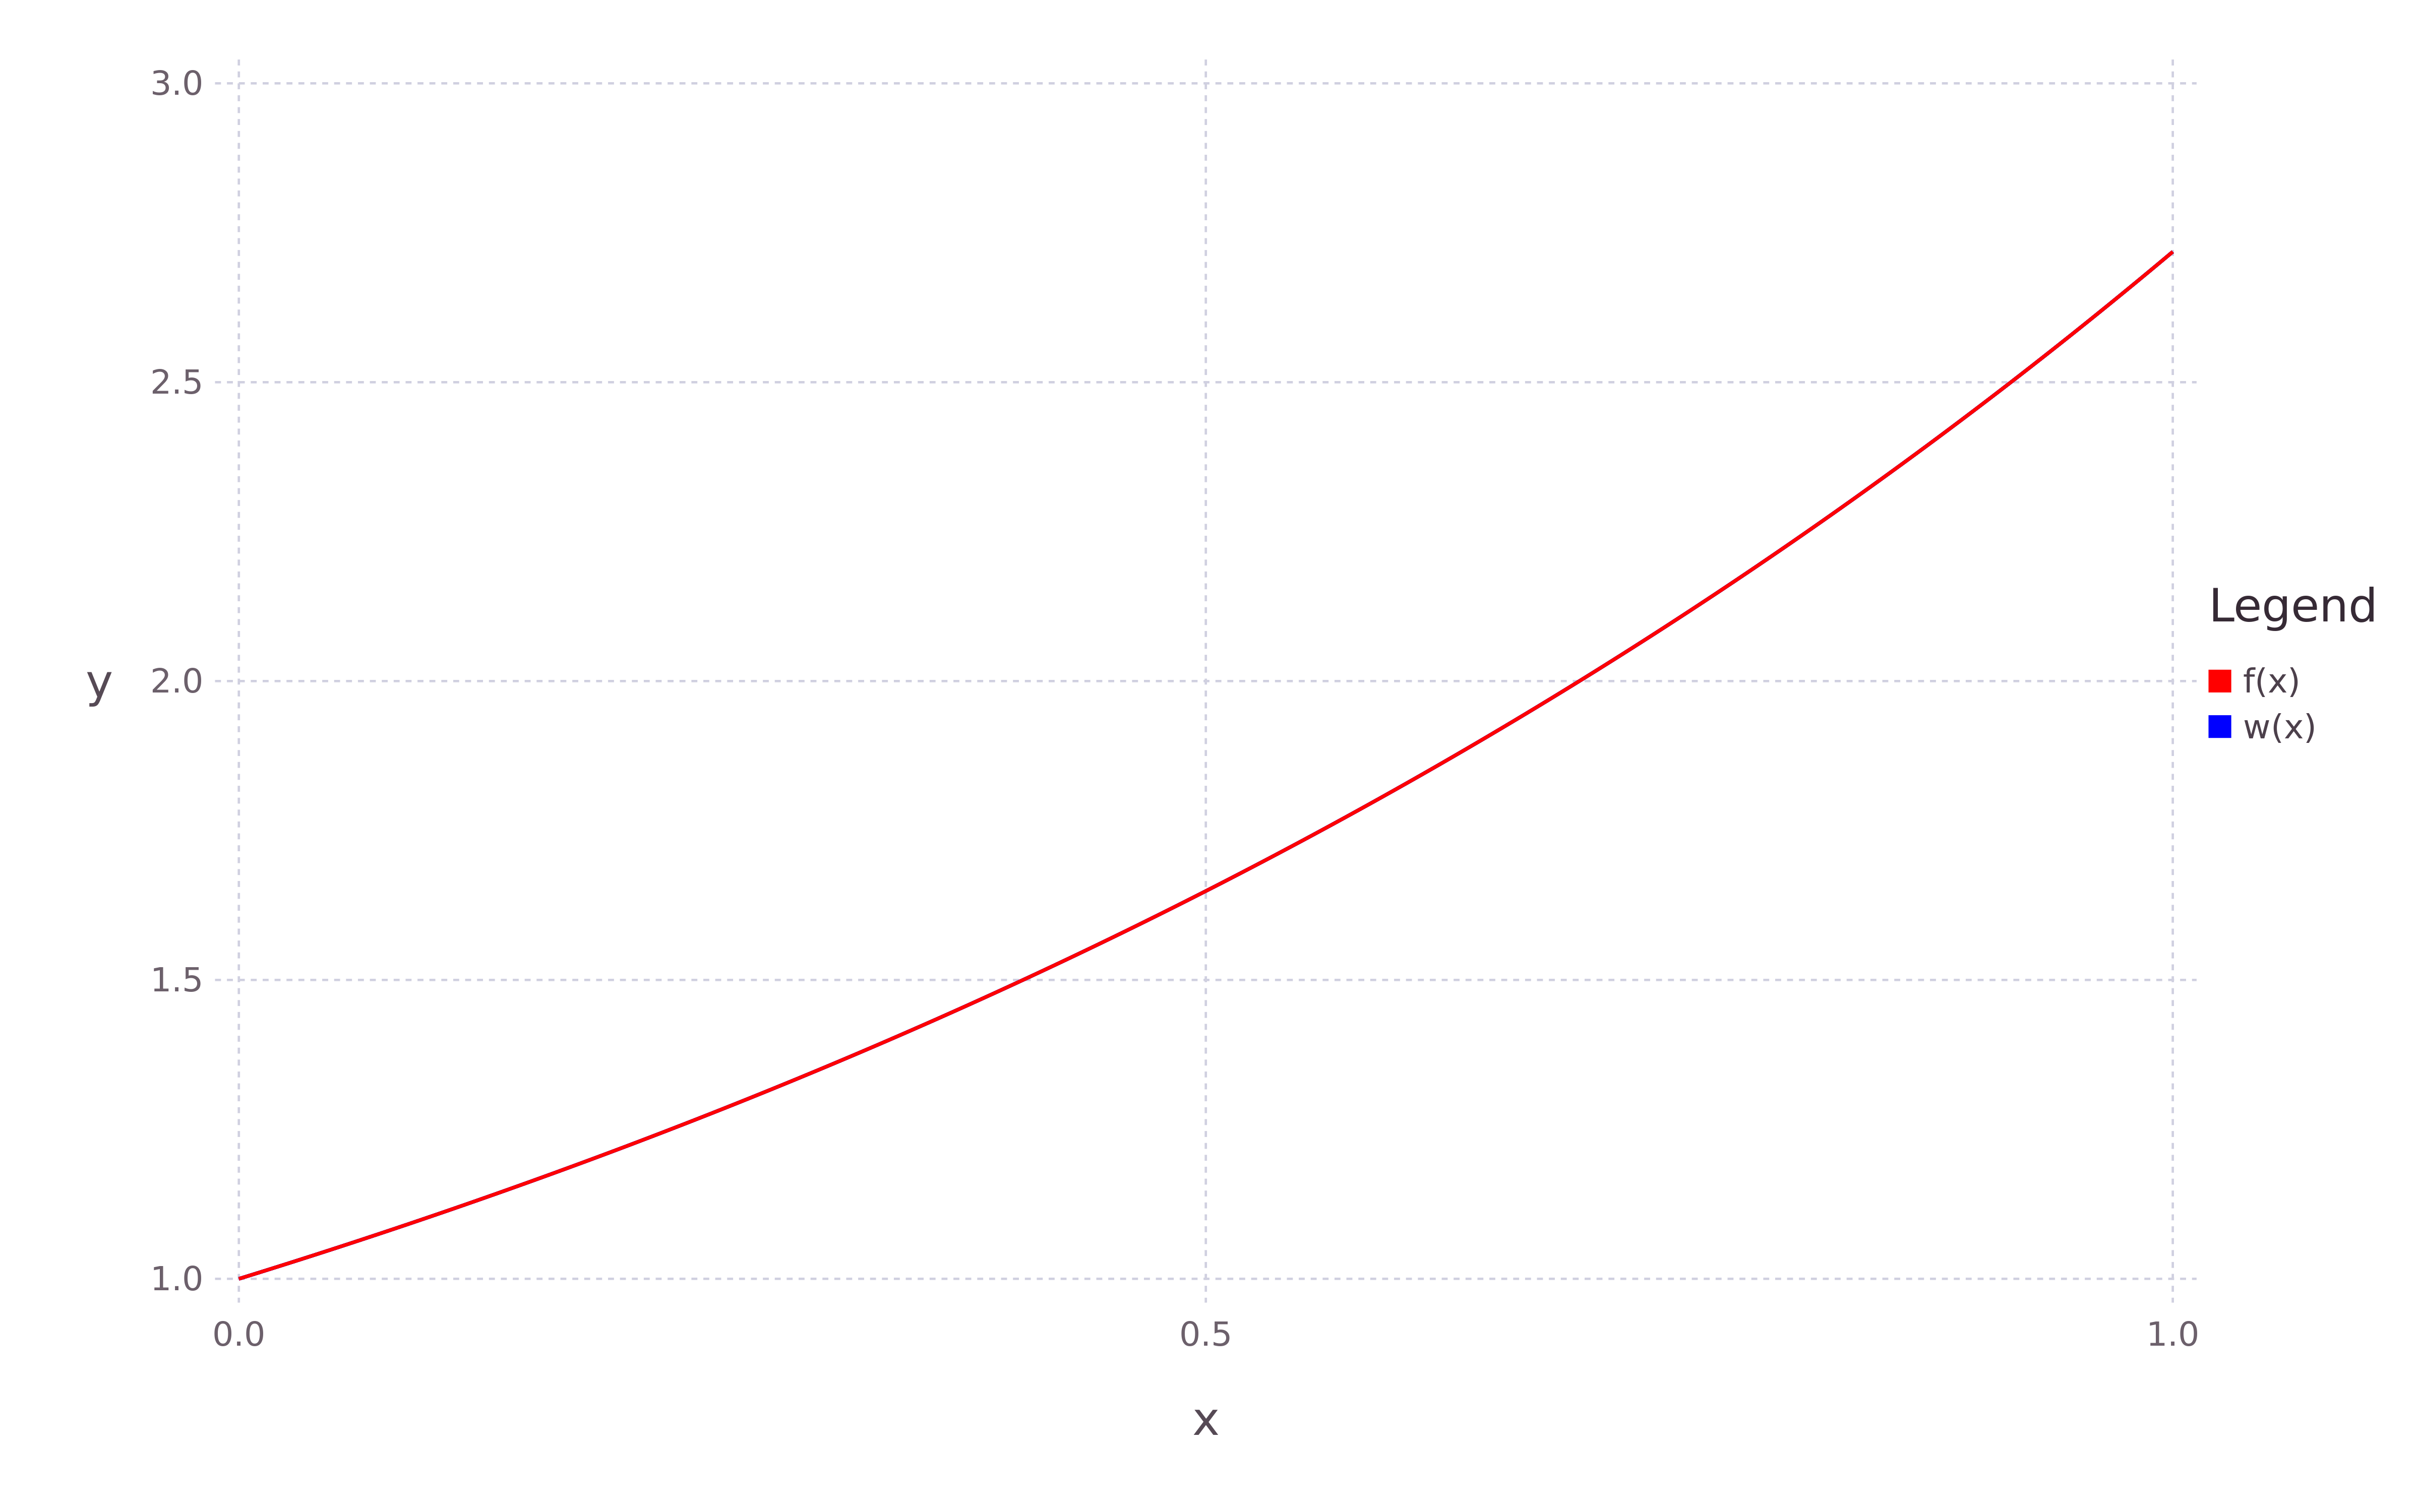
\includegraphics[width=0.5\textwidth]{zad5/plota2.png}} \hfill
			\subfloat[3.][$n=15$]{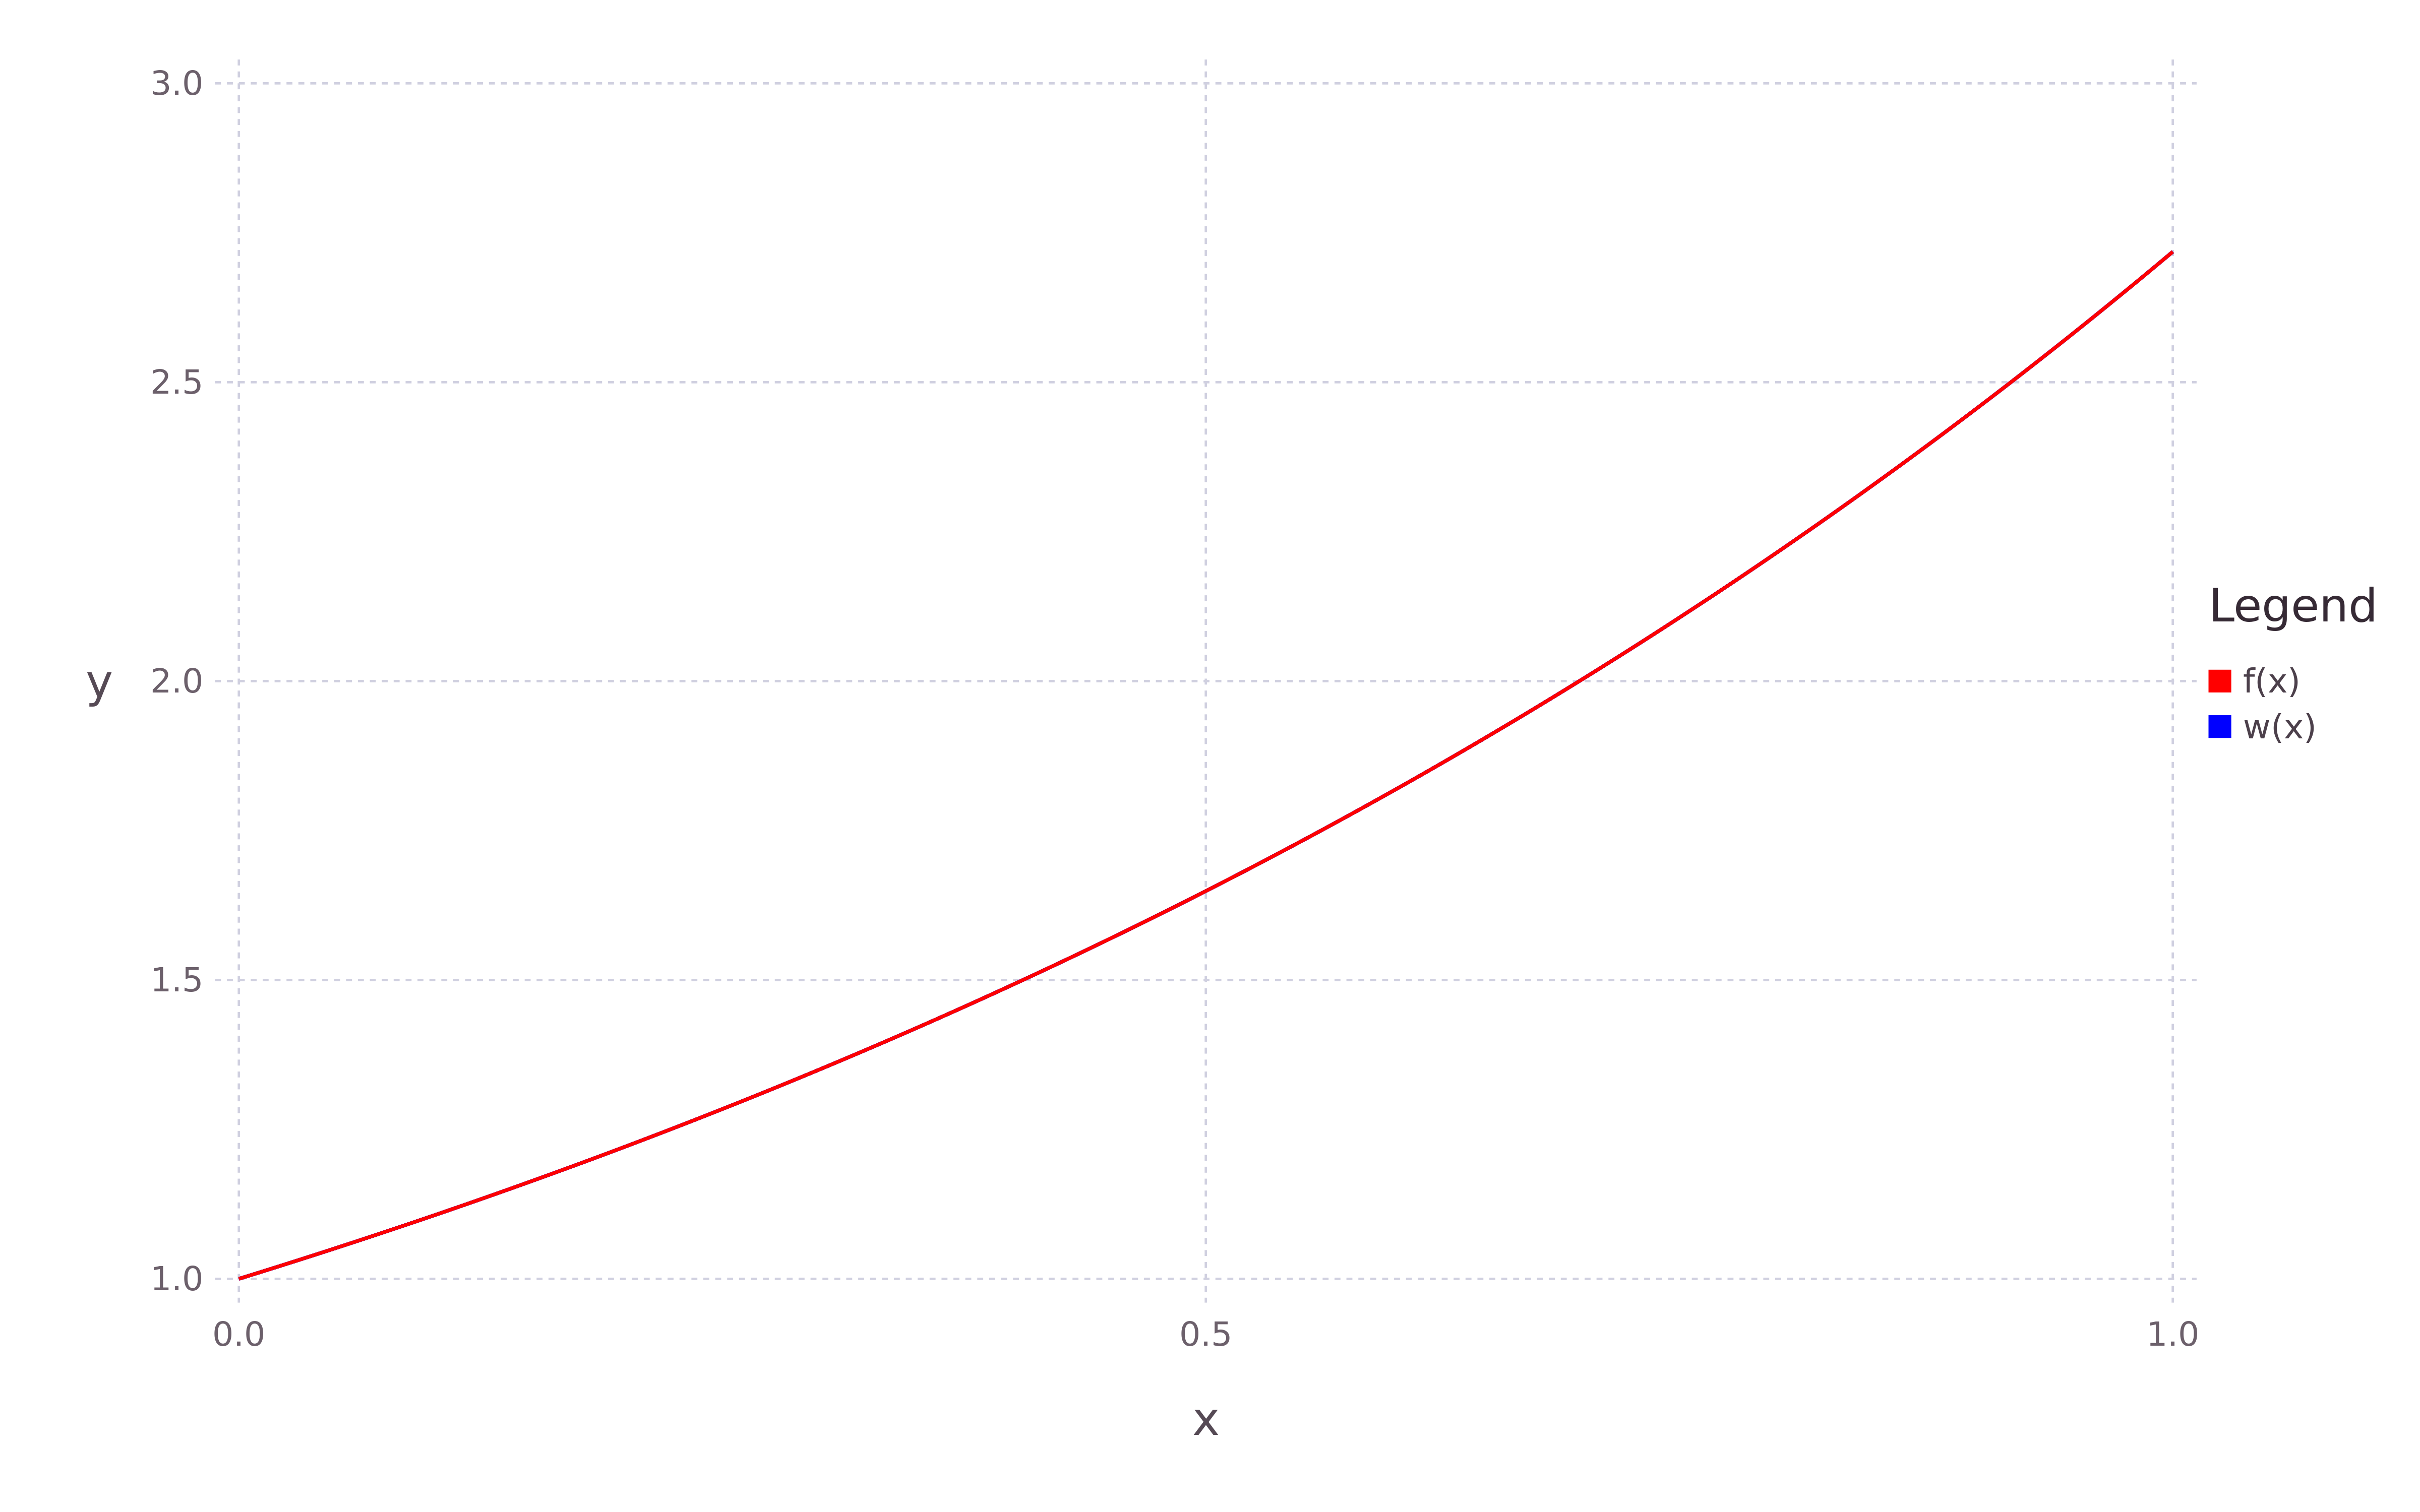
\includegraphics[width=0.5\textwidth]{zad5/plota3.png}}
  			\caption{Wykres funkcji $\exp{x}$ oraz jej wielomianu interpolacyjnego o zadanym stopniu.}
  			\label{fig:1}
		\end{figure}		
		
		\begin{figure}[!h]
			\centering
			\subfloat[1.][$n=5$]{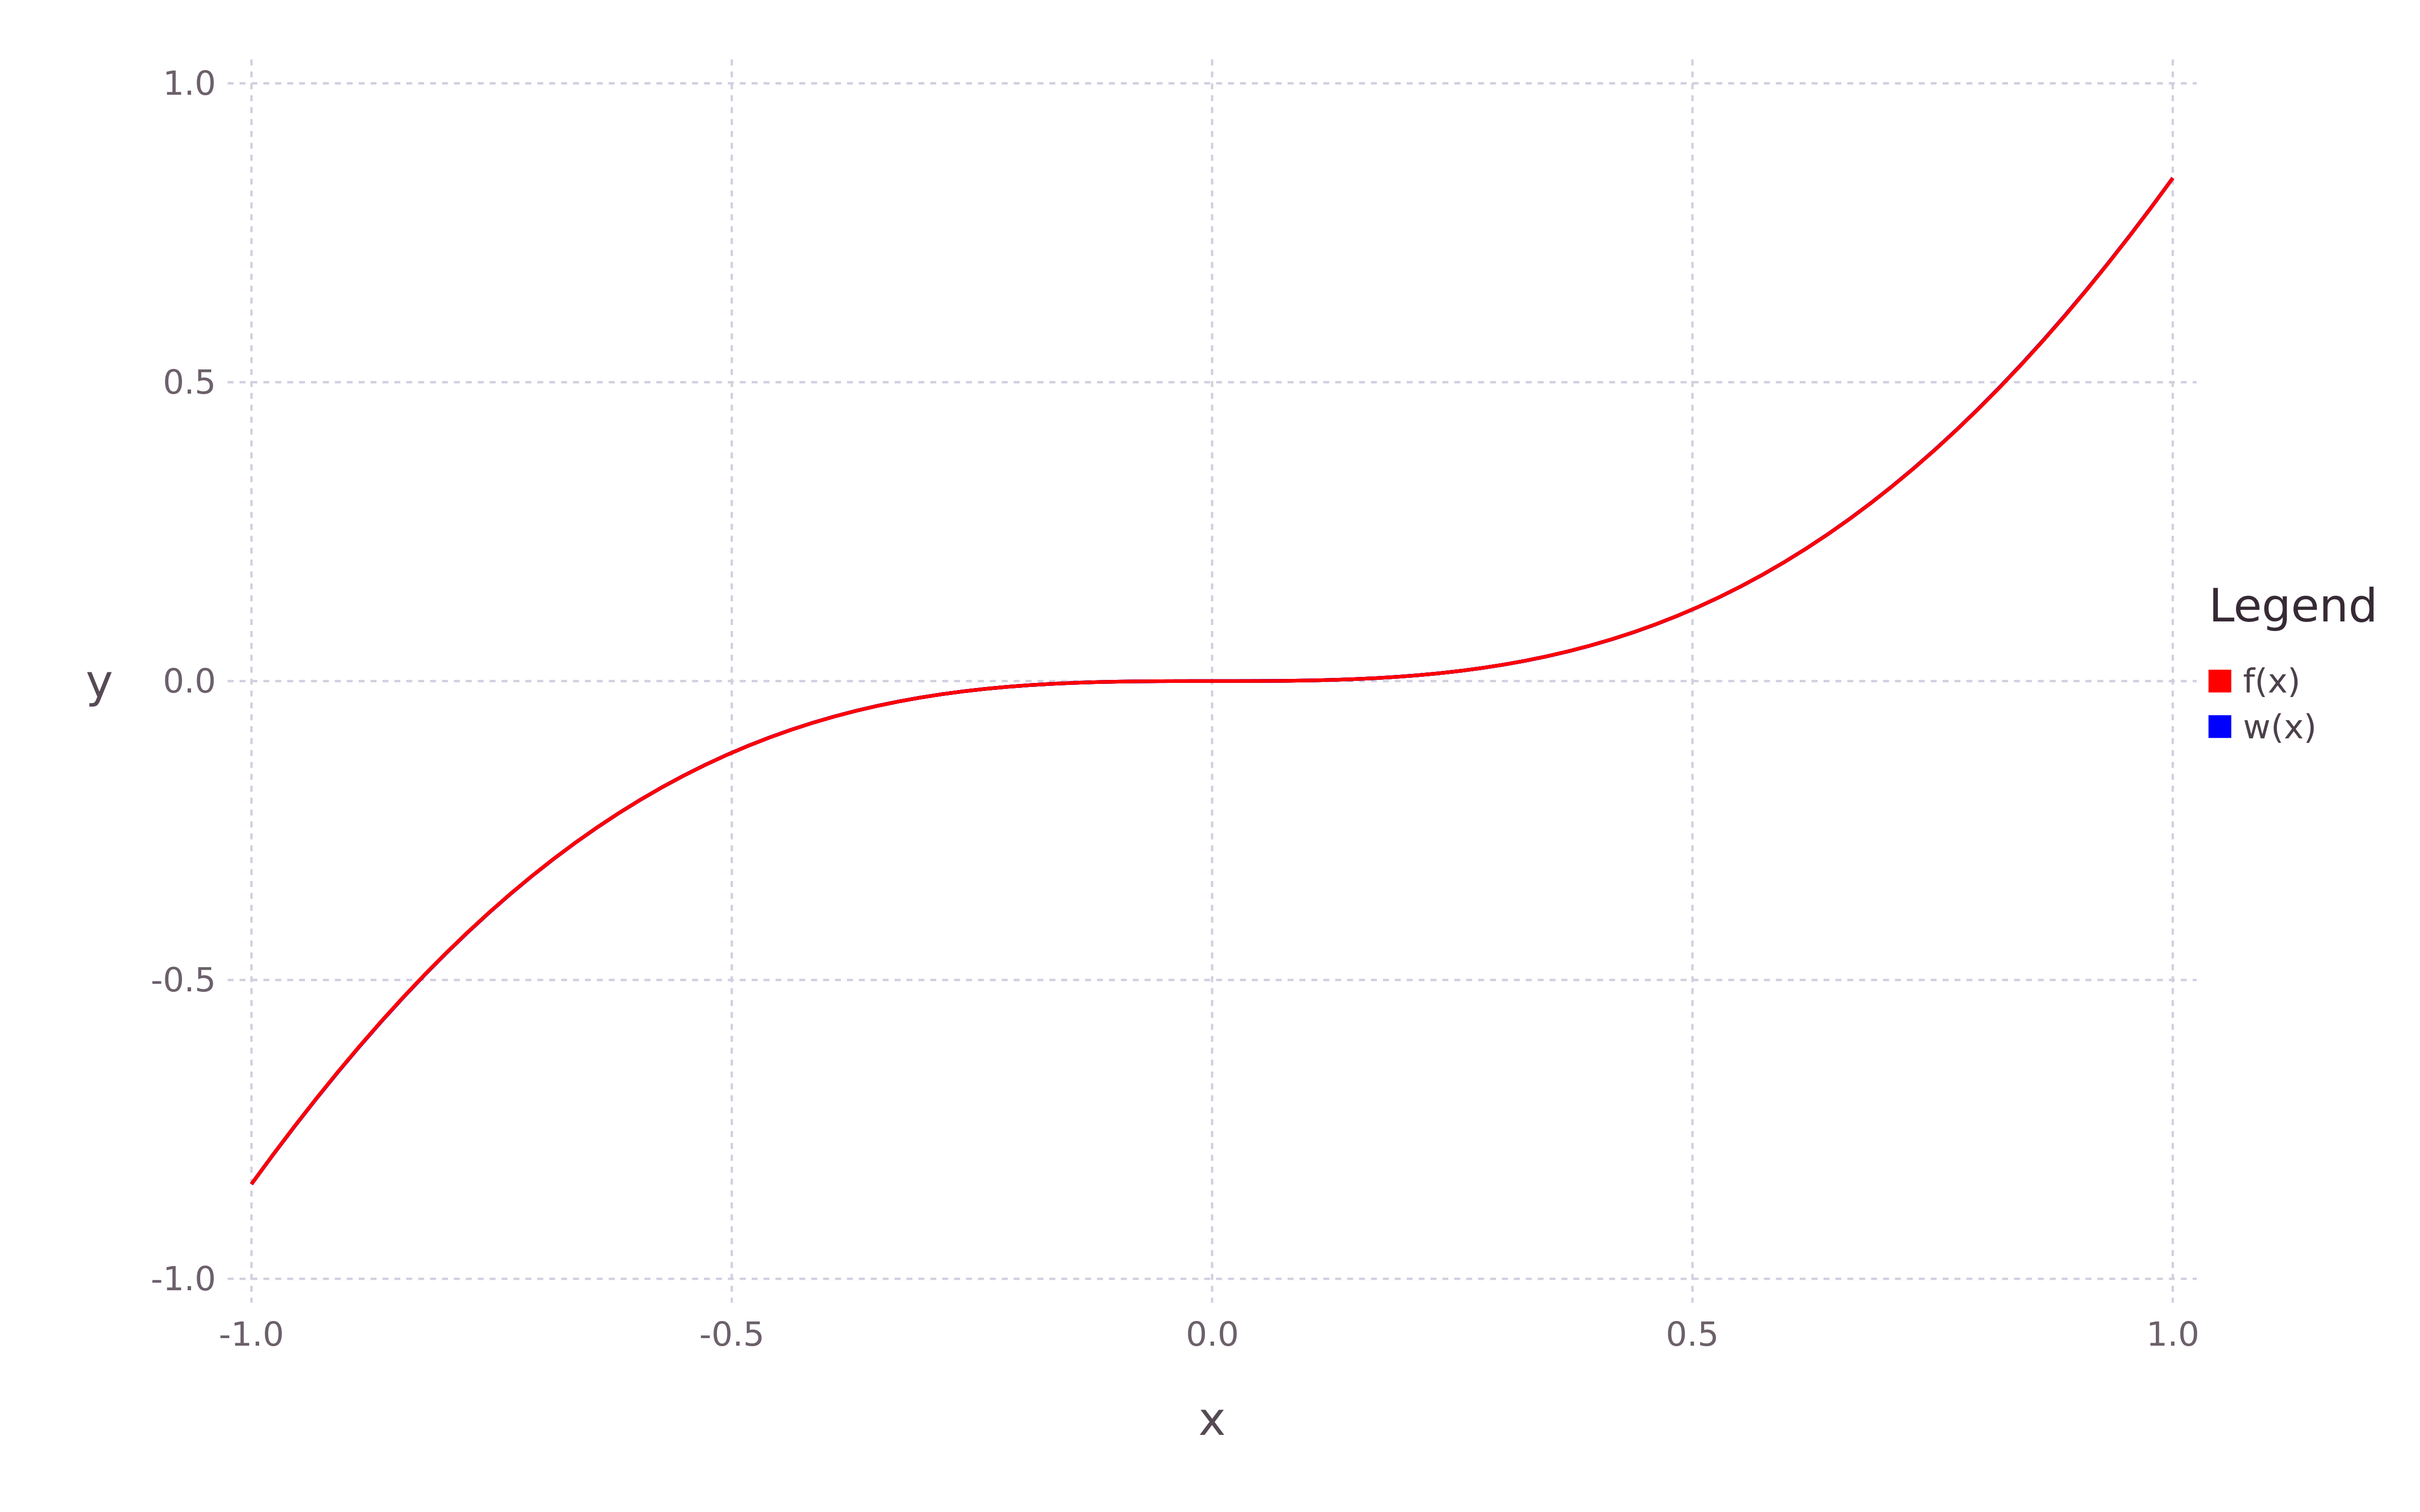
\includegraphics[width=0.5\textwidth]{zad5/plotb1.png}} \hfill
			\subfloat[2.][$n=10$]{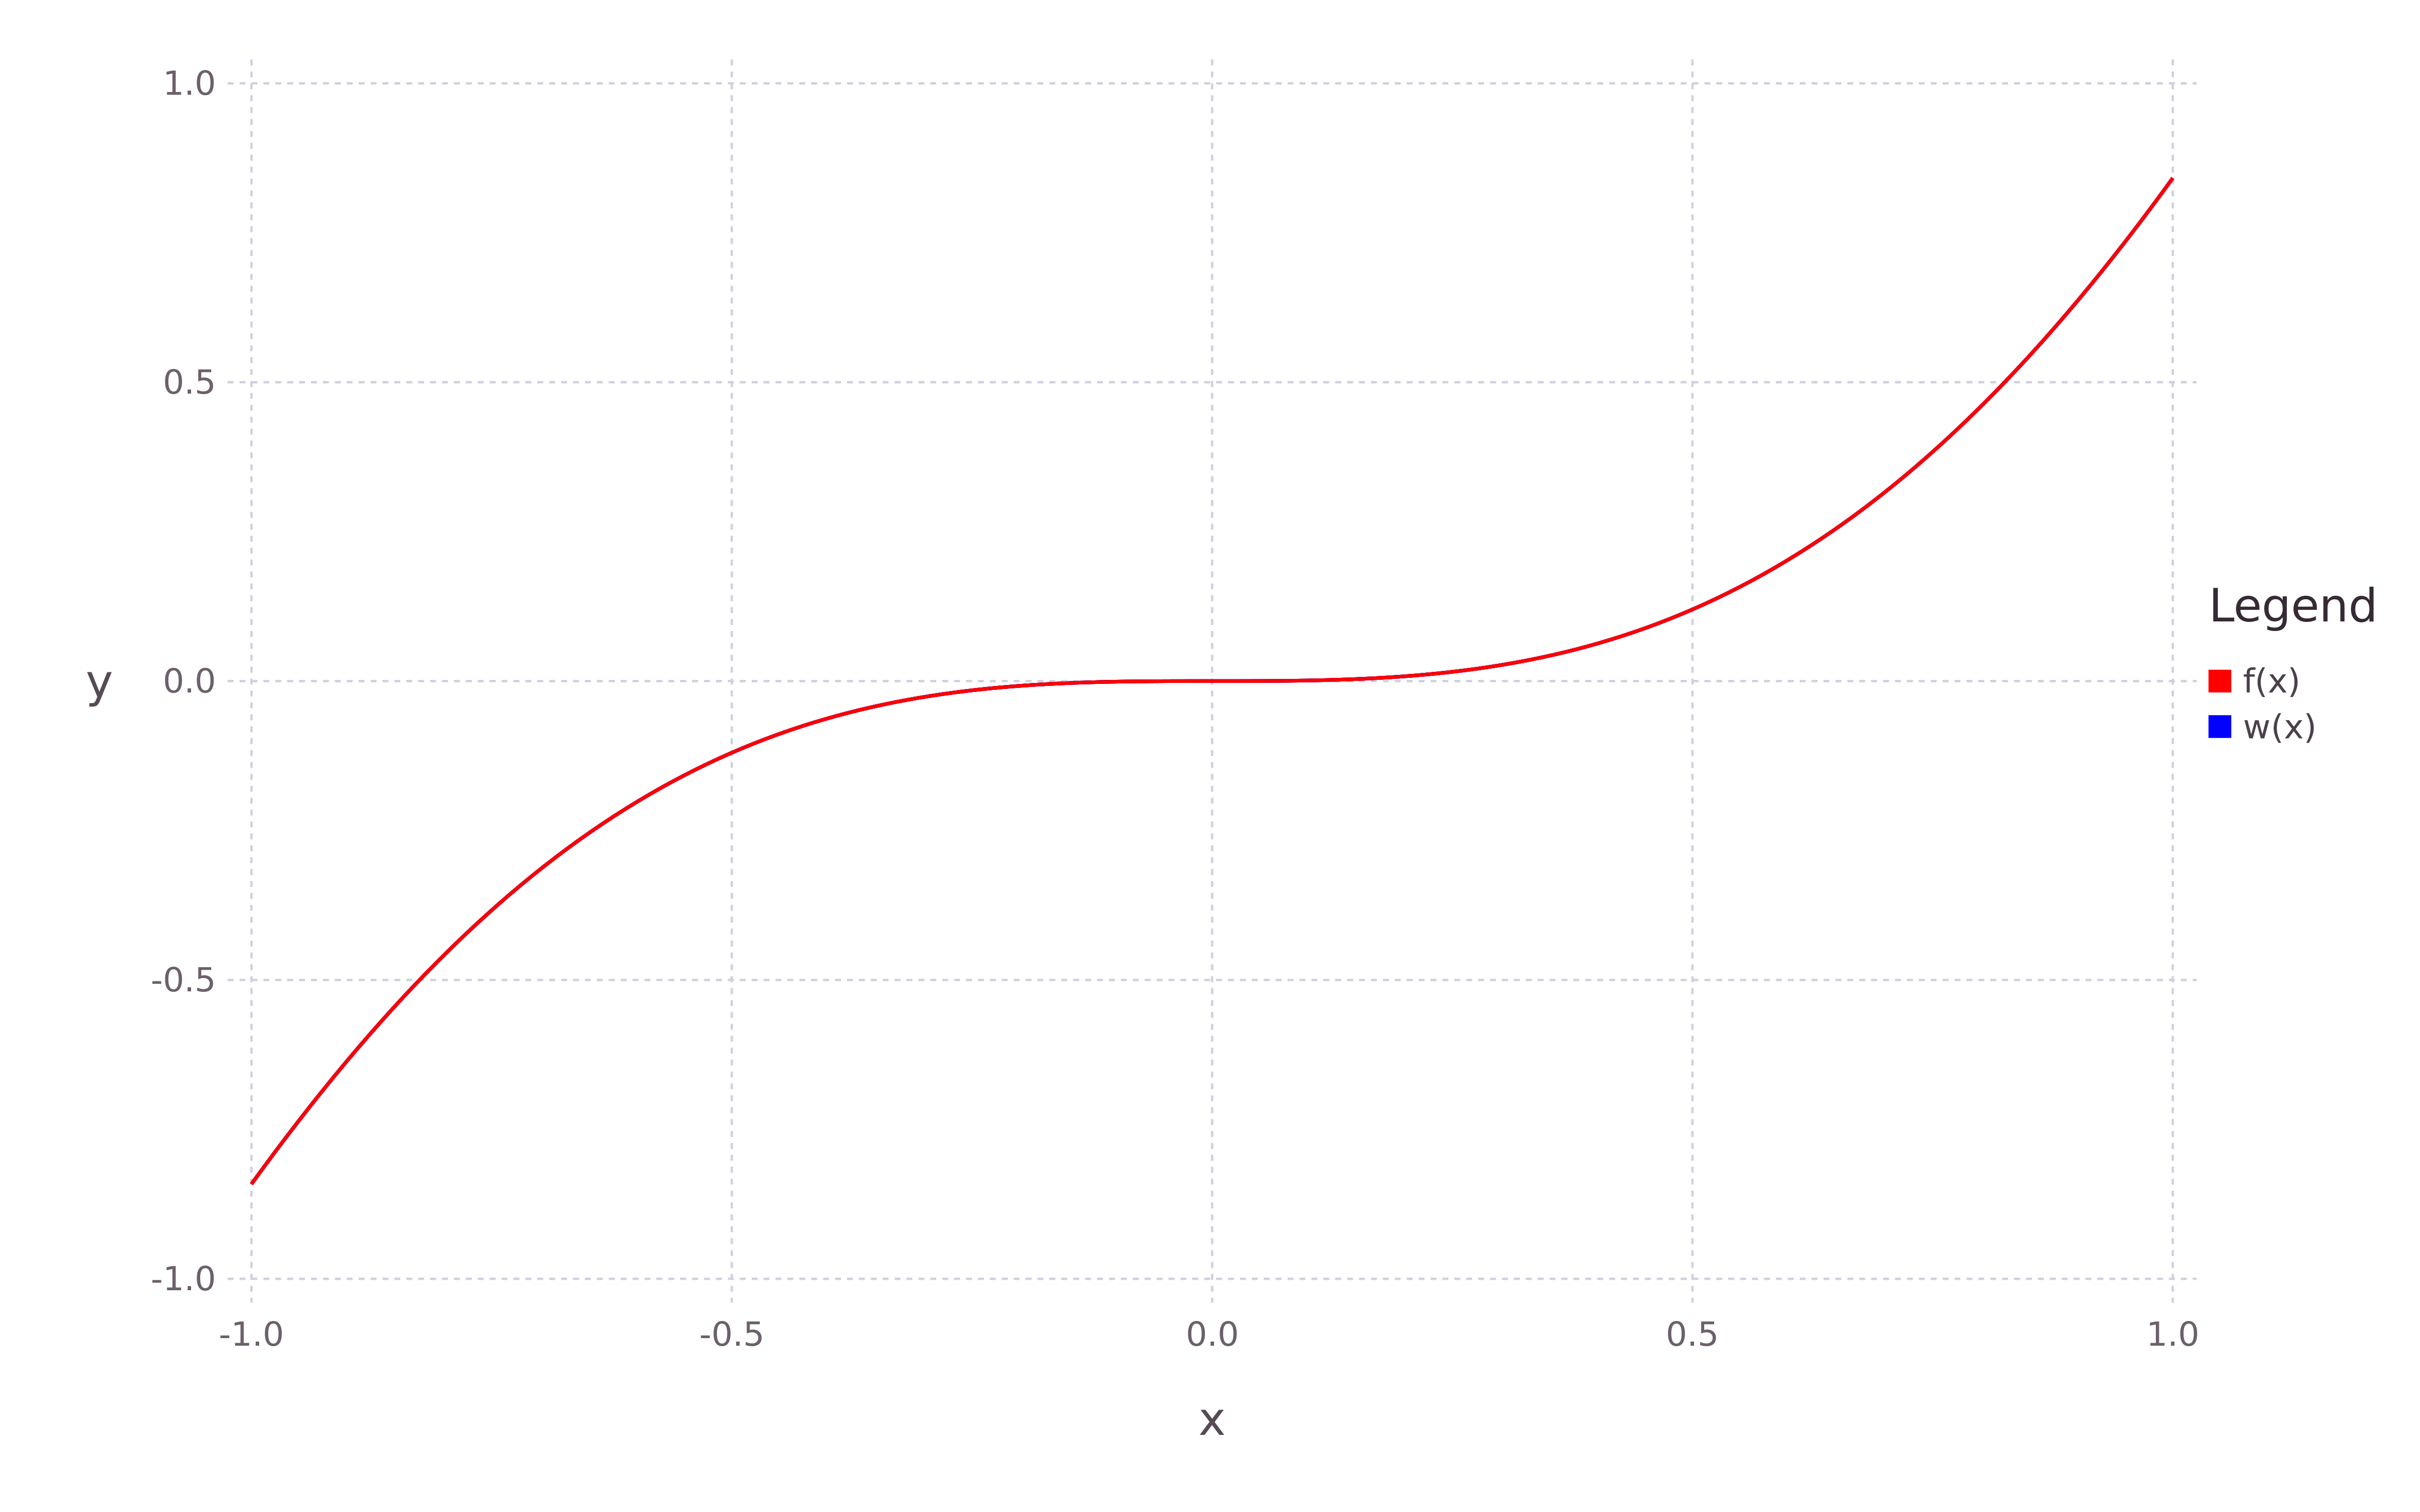
\includegraphics[width=0.5\textwidth]{zad5/plotb2.png}} \hfill
			\subfloat[3.][$n=5$]{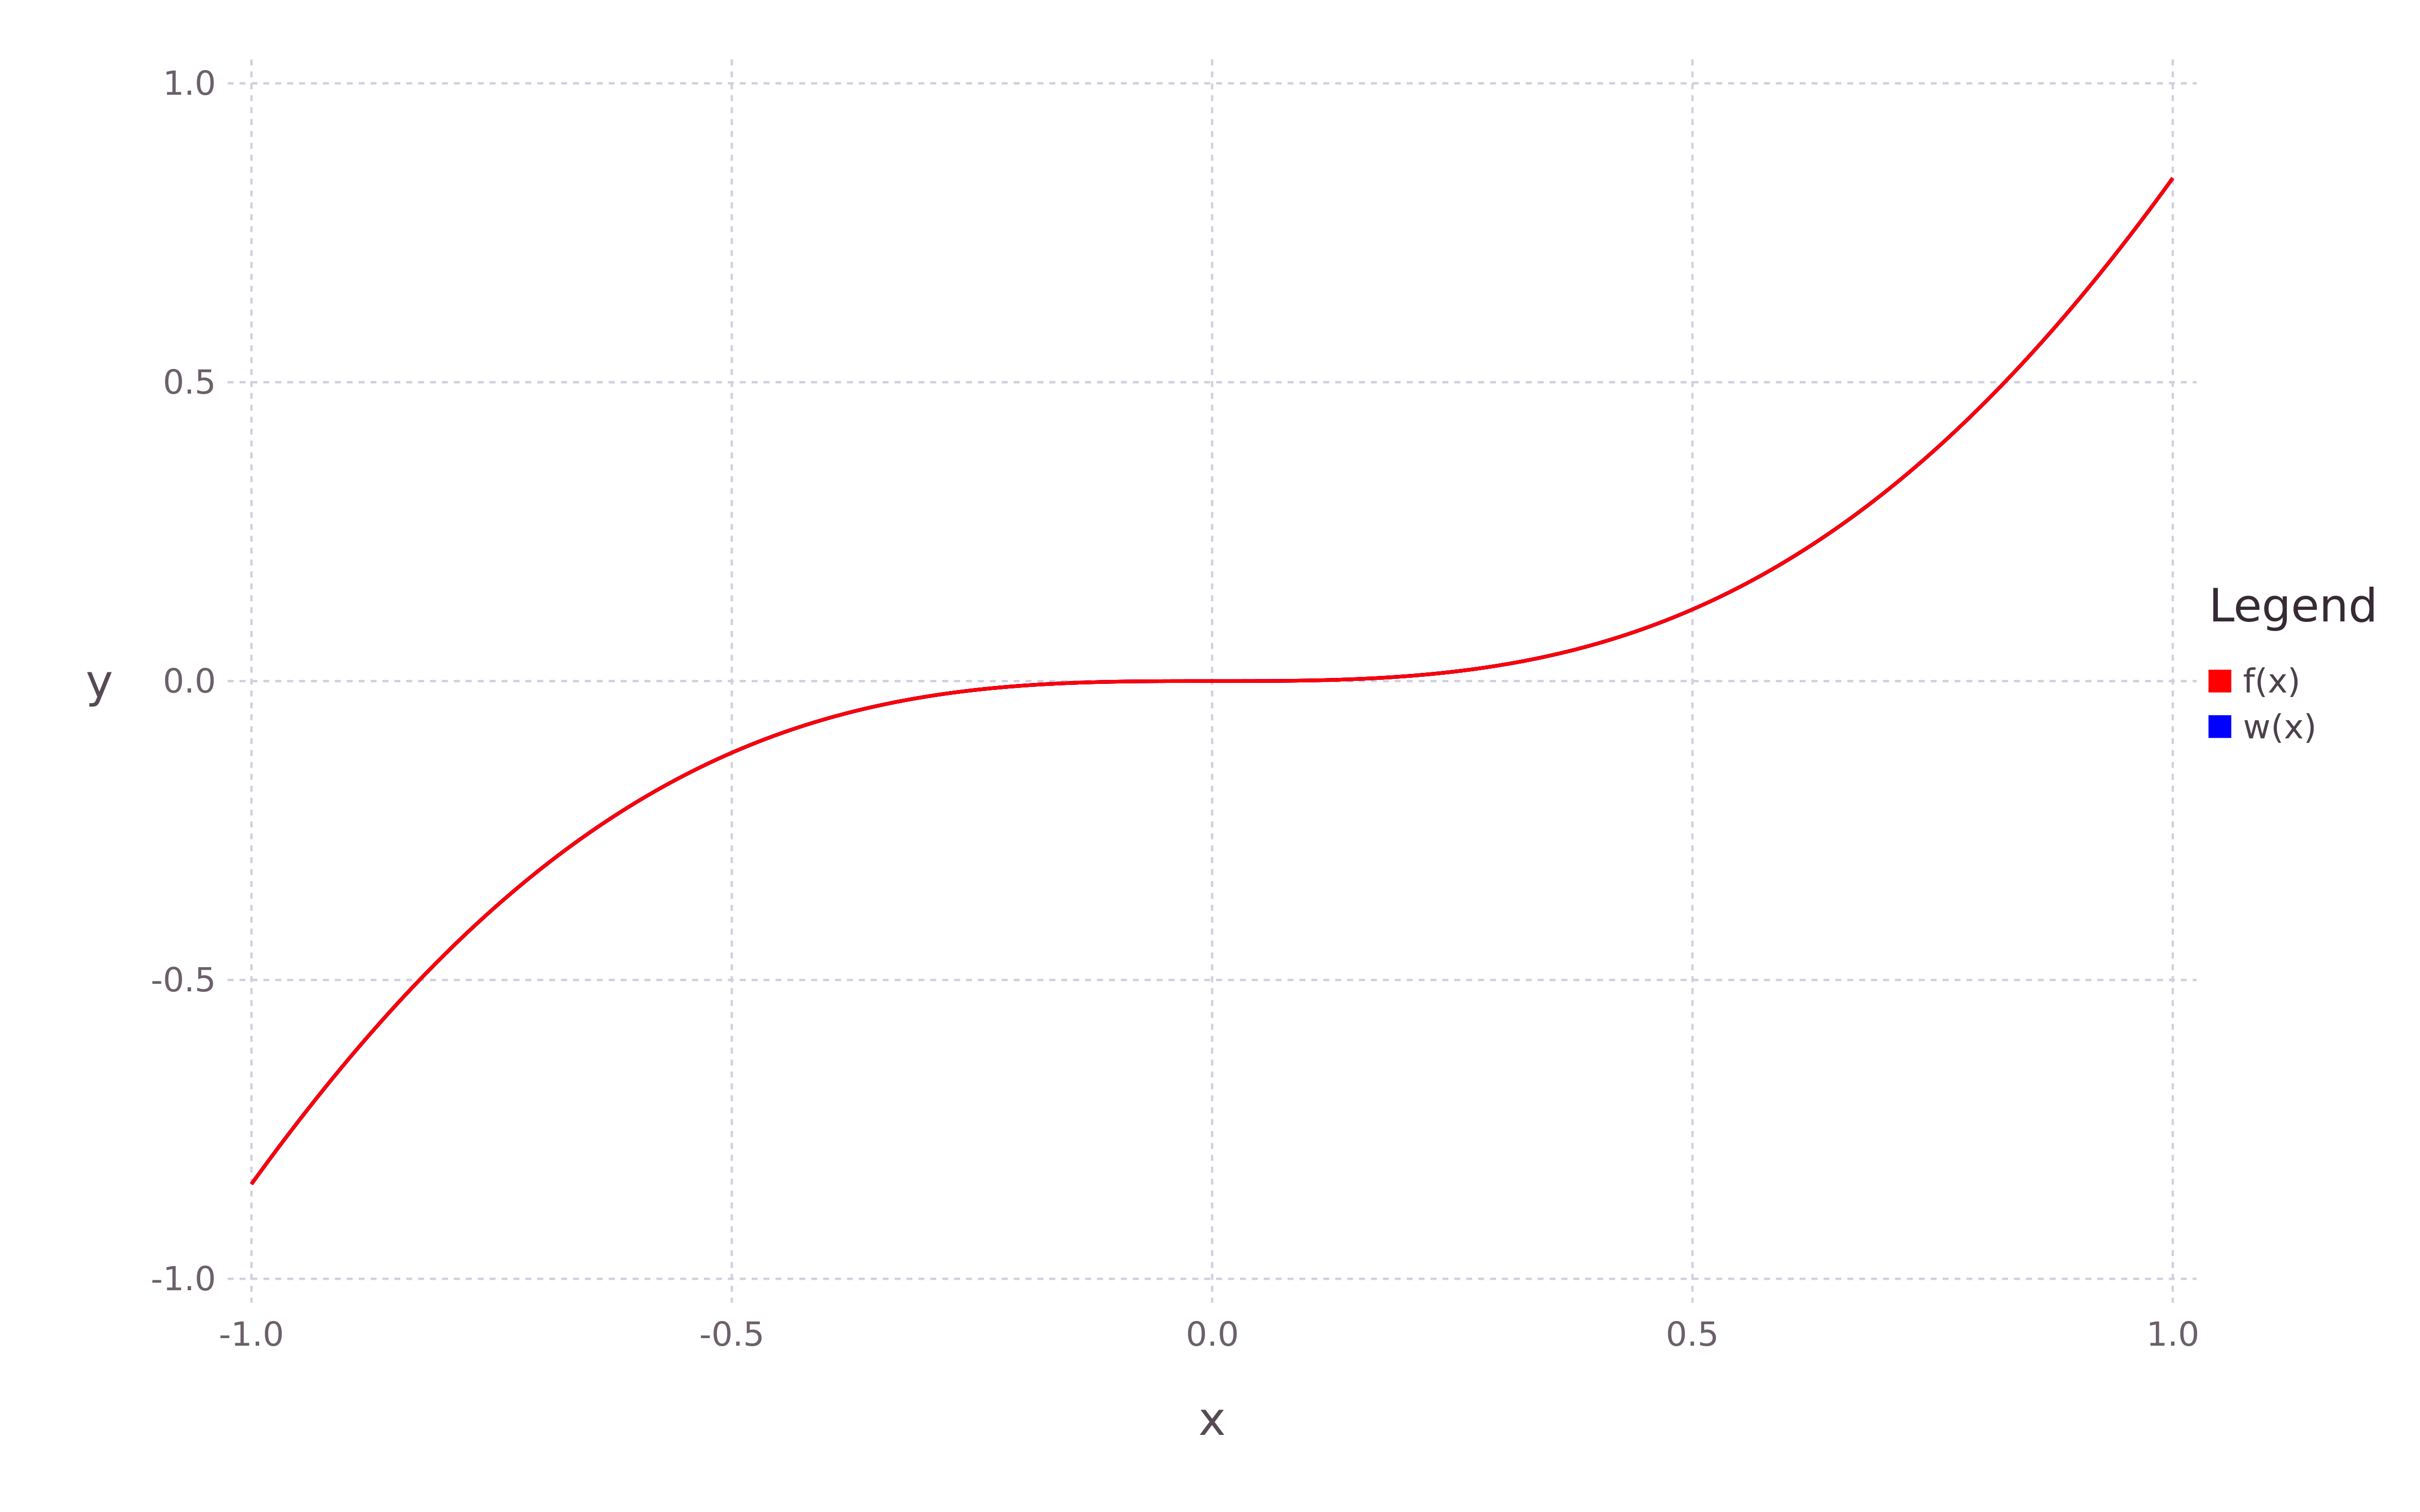
\includegraphics[width=0.5\textwidth]{zad5/plotb3.png}}
  			\caption{Wykres funkcji $x^2 \cdot \sin{x}$ oraz jej wielomianu interpolacyjnego o zadanym stopniu.}
  			\label{fig:2}
		\end{figure}	
		
	\subsection{Wnioski}
		Analiza przedstawionych powyżej wykresów pozwala na zaobserwowanie braku rozbieżności w przypadku obu funkcji --- na zadanych przedziałach wielomiany interpolacyjne niemal pokrywają się z odpowiadającą funkcją. Już w przypadku wielomianu o stopniu $n=5$ powstałe różnice są rzędu $10^{-6}$, malejąc wraz ze zwiększaniem stopnia. W tych konkretnych przypadkach zastosowanie równoodległych węzłów interpolacji (na których to użyciu oparto rozwiązanie Zadania 4.) poskutkowało uzyskaniem niezwykle dobrych przybliżeń.
	
\section{Zadanie 6}	
	\subsection{Opis problemu}
		Celem zadania było przetestowanie utworzonej w Zadaniu 4 funkcji \texttt{rysujNnfx} na następujących przykładach:
			\begin{enumerate}[(a)]
				\item $|x|,~ [-1,1],~ n = 5, 10, 15$,
				\item $\frac{1}{1+x^2},~ [-5,5],~ n = 5, 10, 15$.
			\end{enumerate}
	\subsection{Opis rozwiązania}
		Funkcję \texttt{rysujNnfx} wywołano dla powyższych danych.
	\subsection{Wyniki}	
		Uzyskane wykresy przedstawiono na Rysunkach \ref{fig:3}-\ref{fig:4}.	
	
		\begin{figure}[!h]
			\centering
			\subfloat[1.][$n=5$]{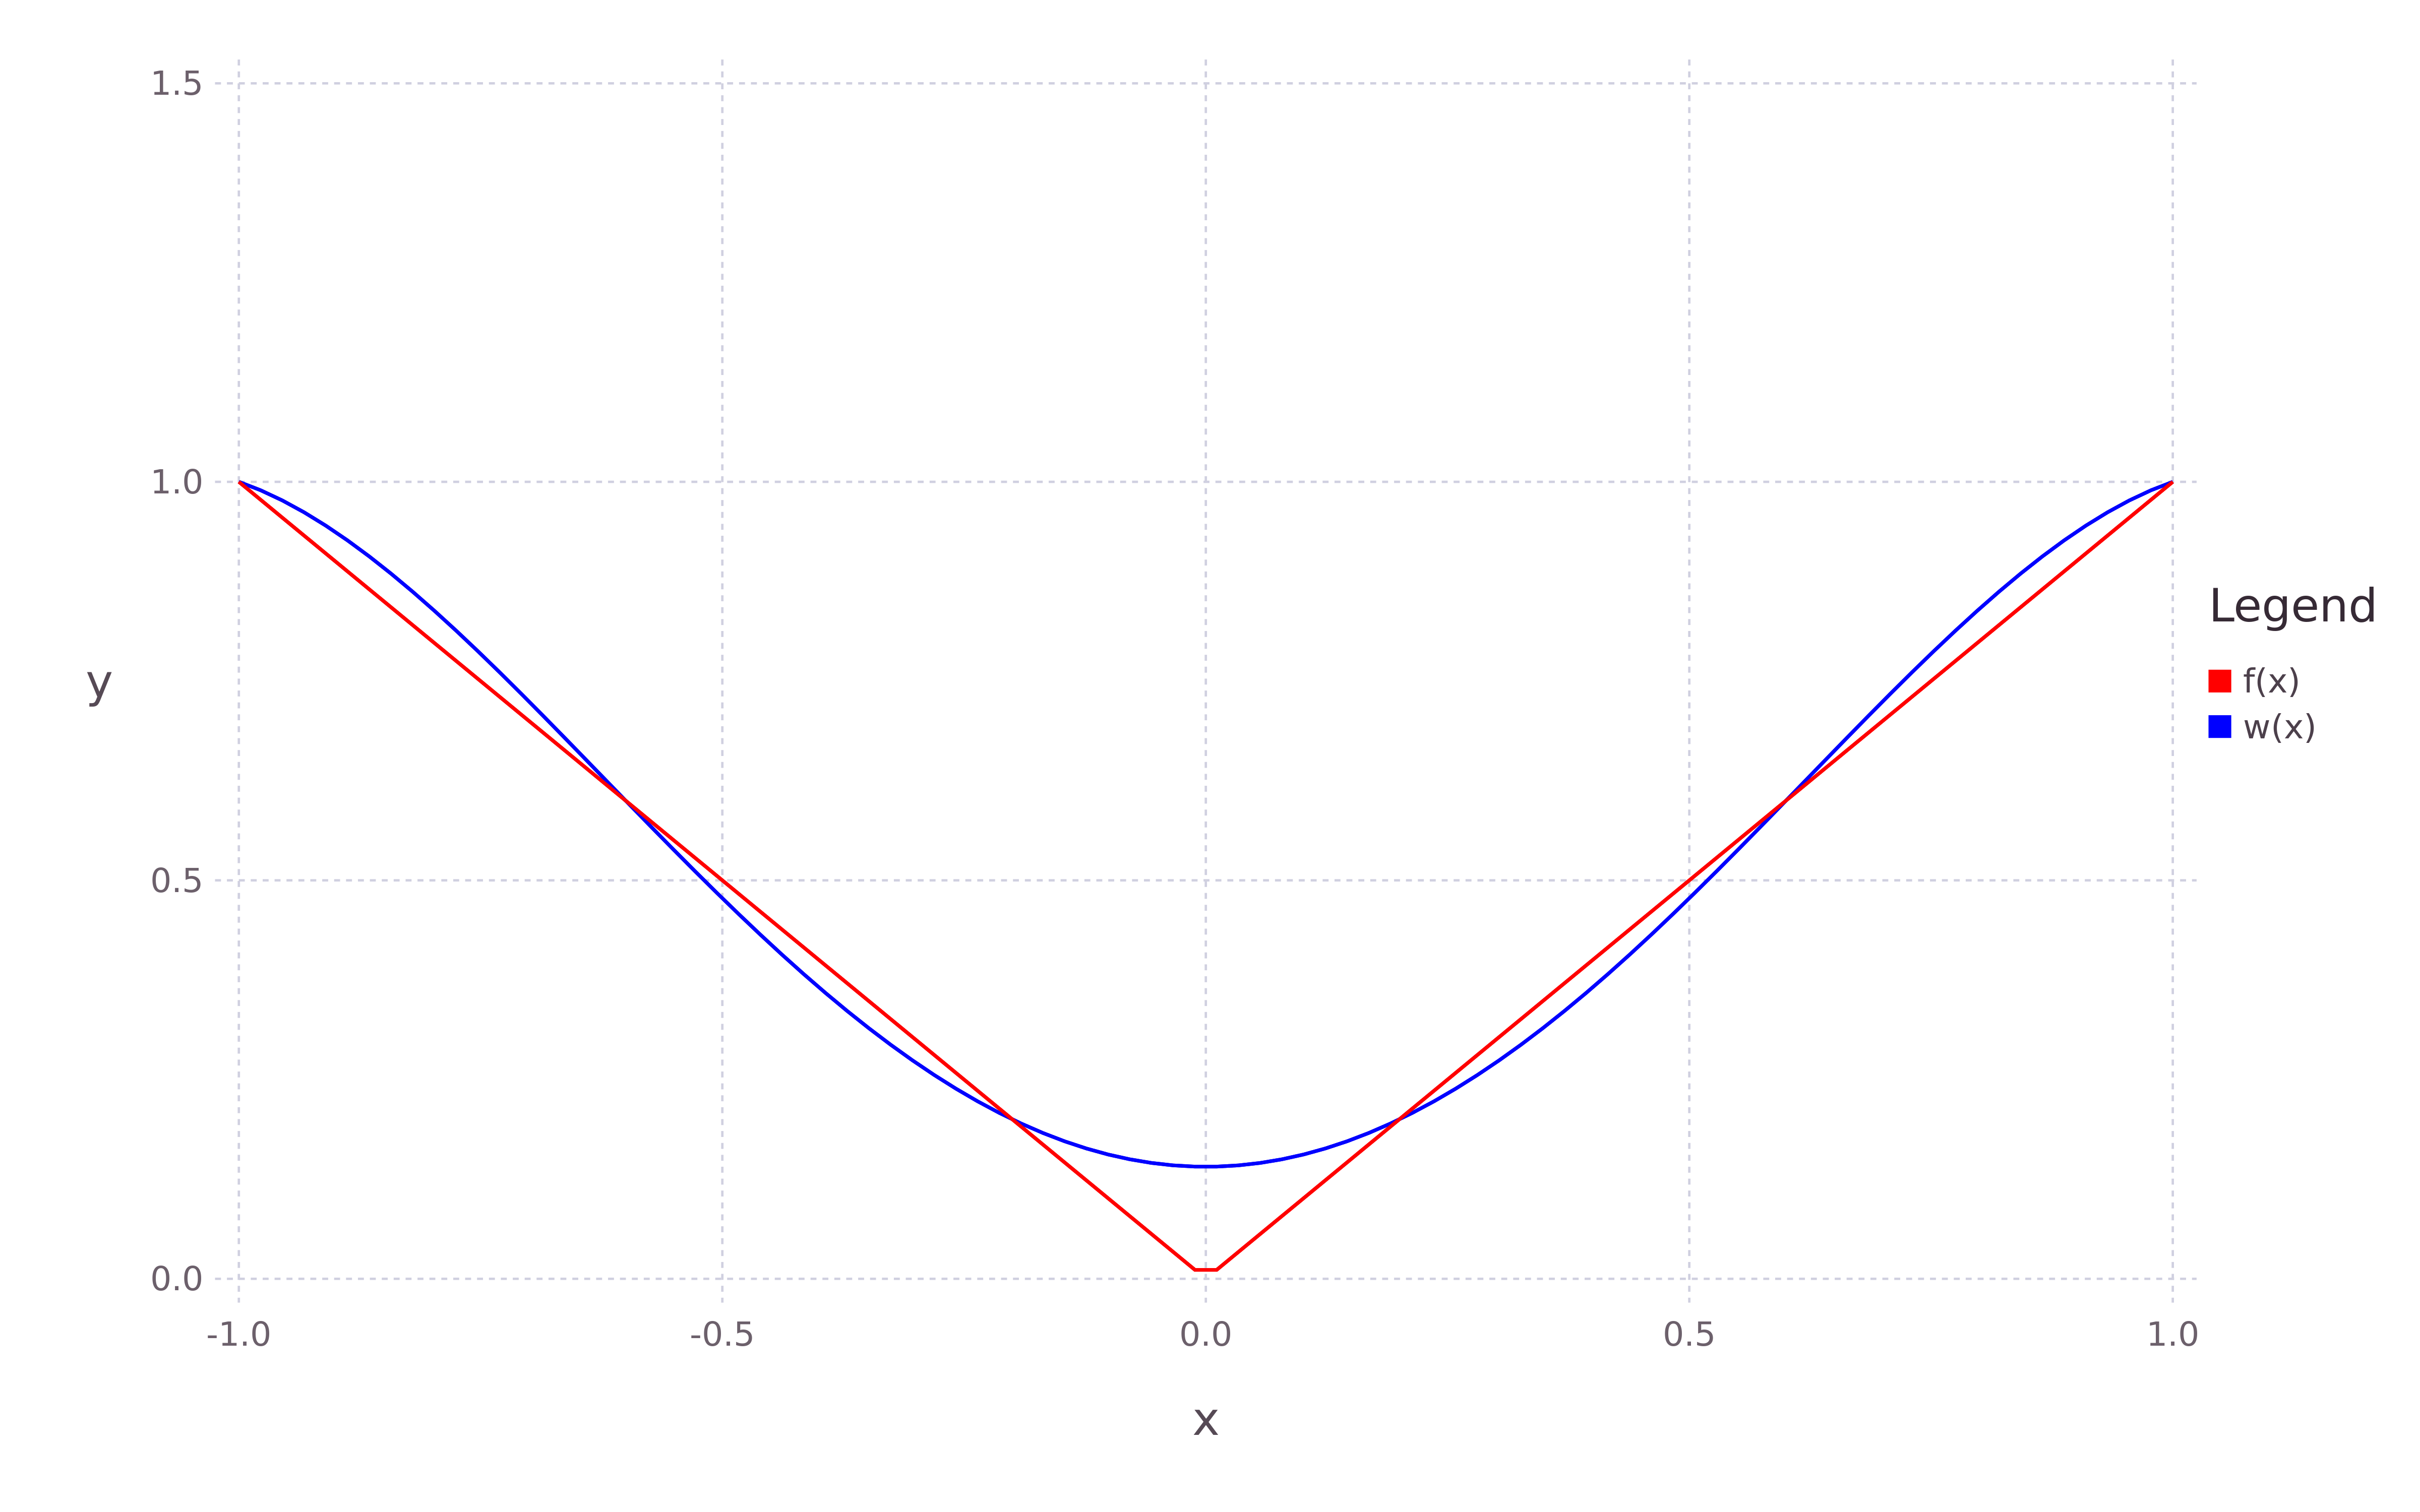
\includegraphics[width=0.5\textwidth]{zad6/plota1.png}} \hfill
			\subfloat[2.][$n=10$]{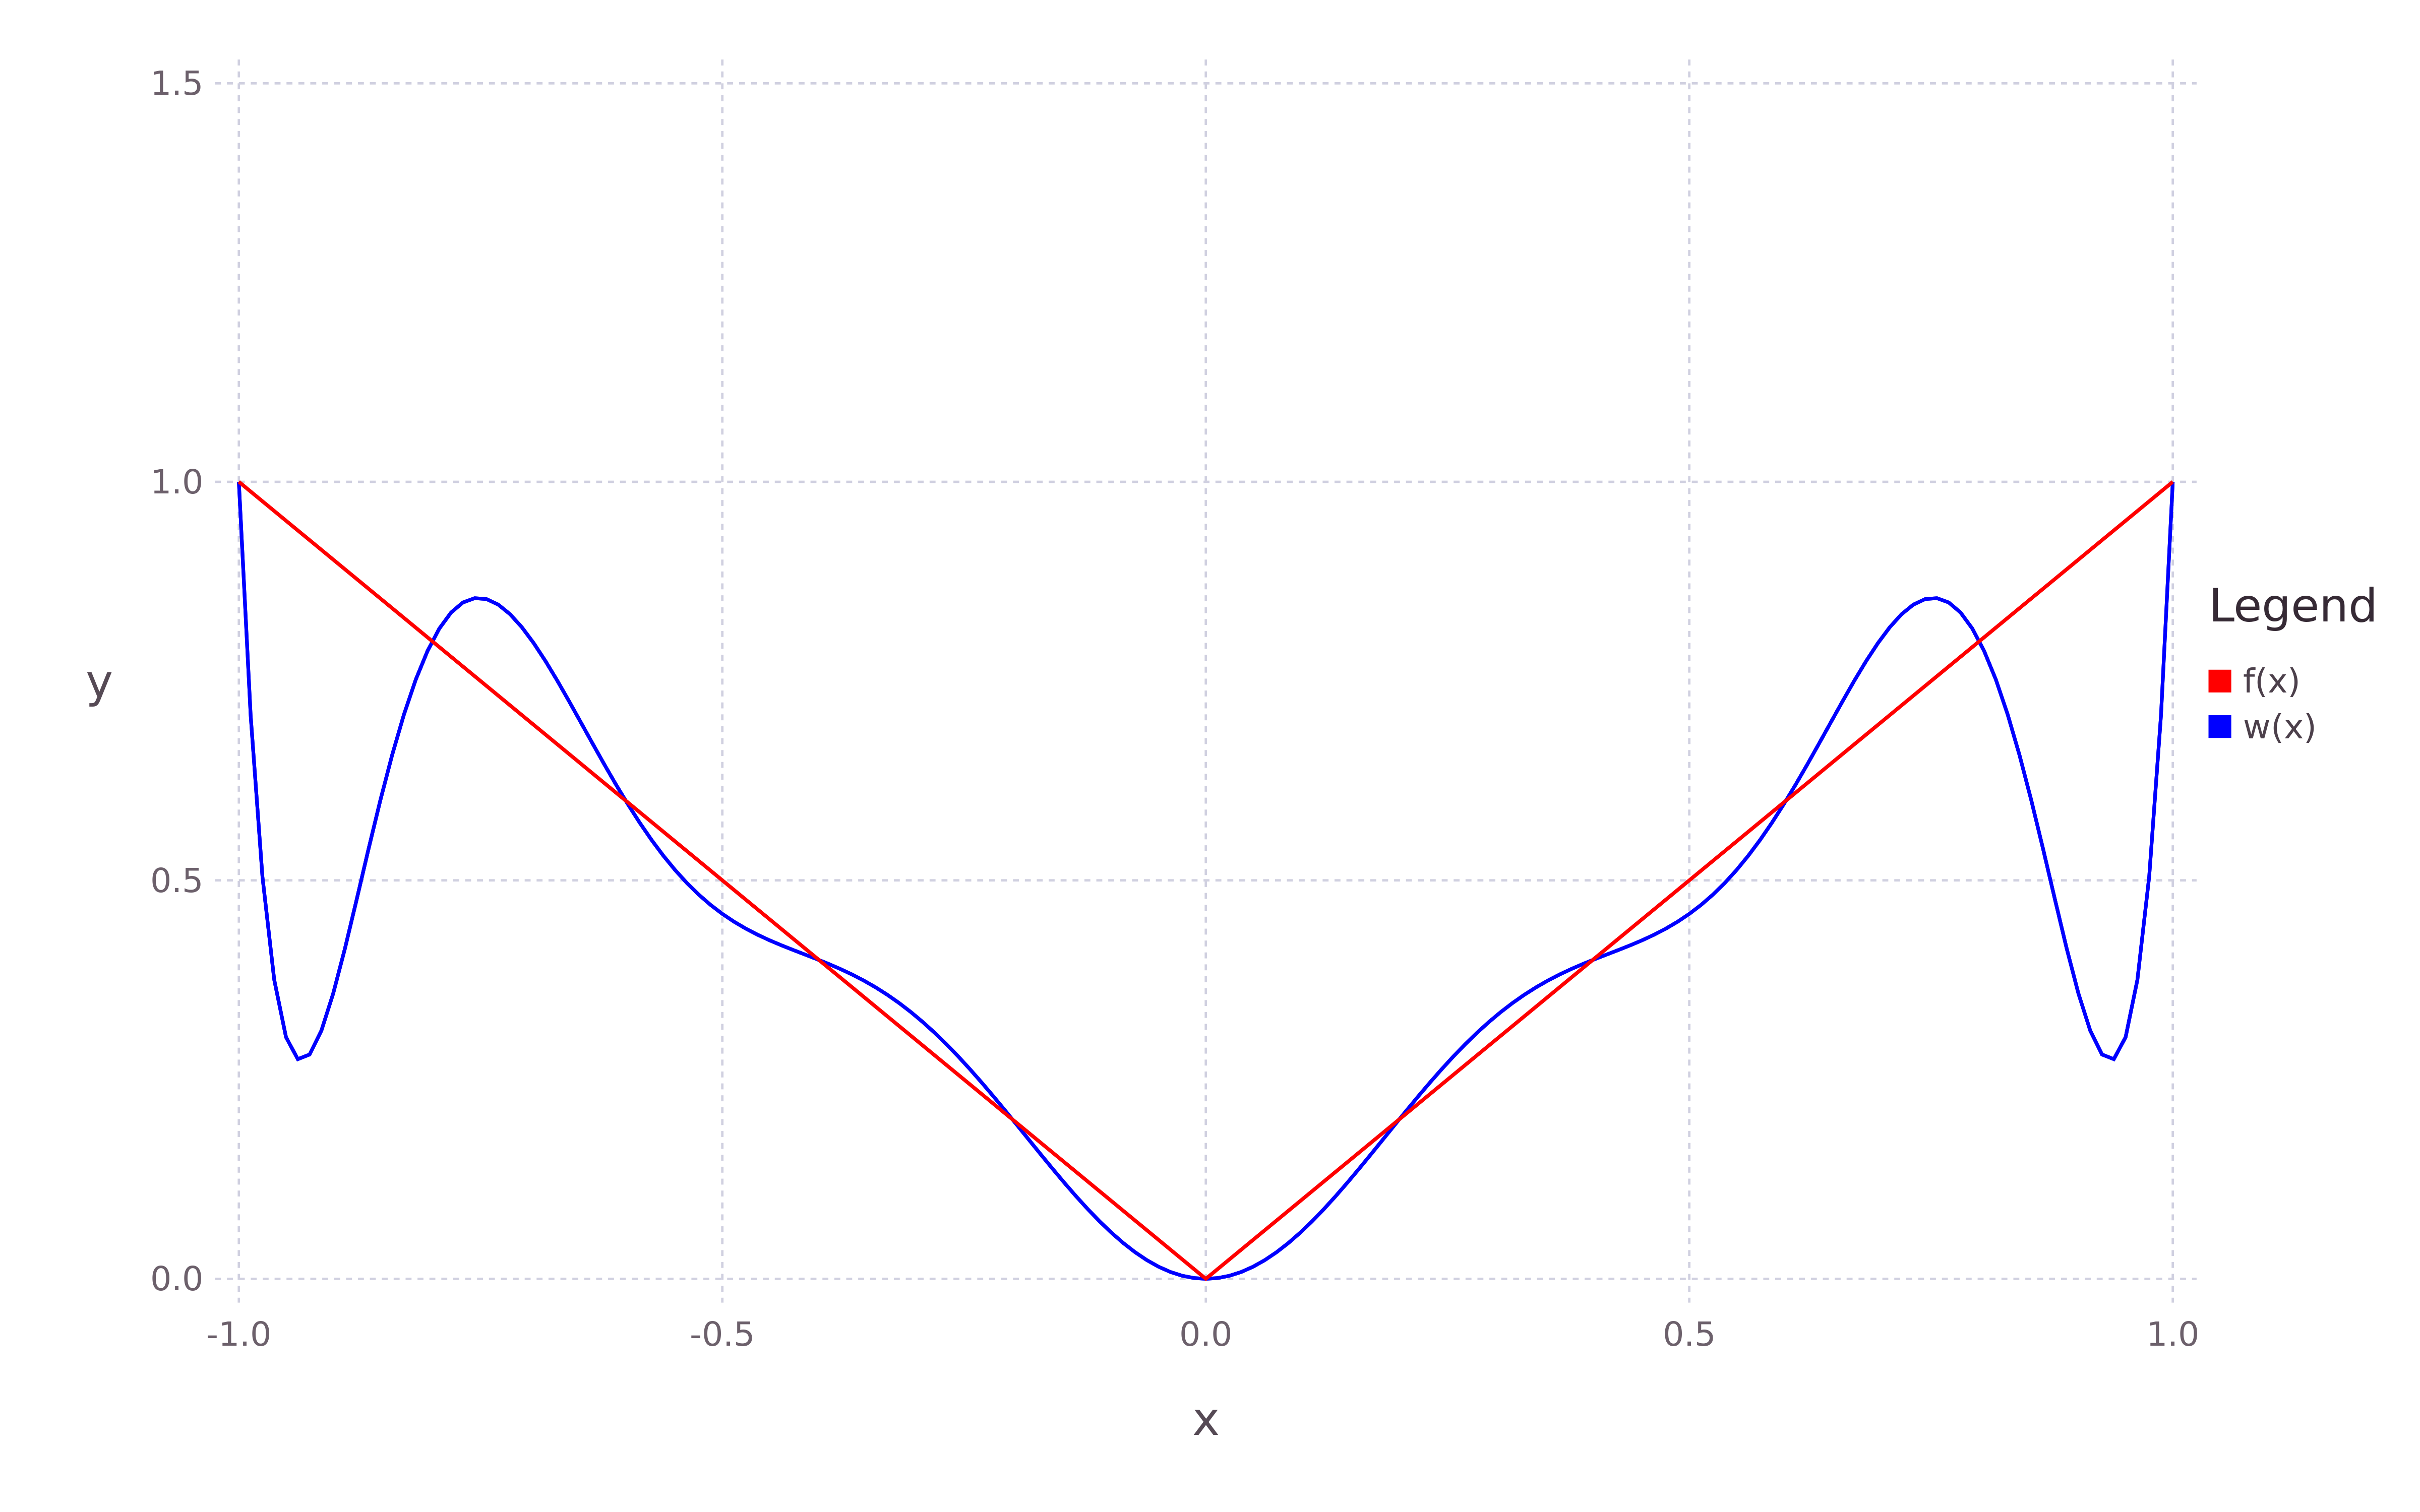
\includegraphics[width=0.5\textwidth]{zad6/plota2.png}} \hfill
			\subfloat[3.][$n=15$]{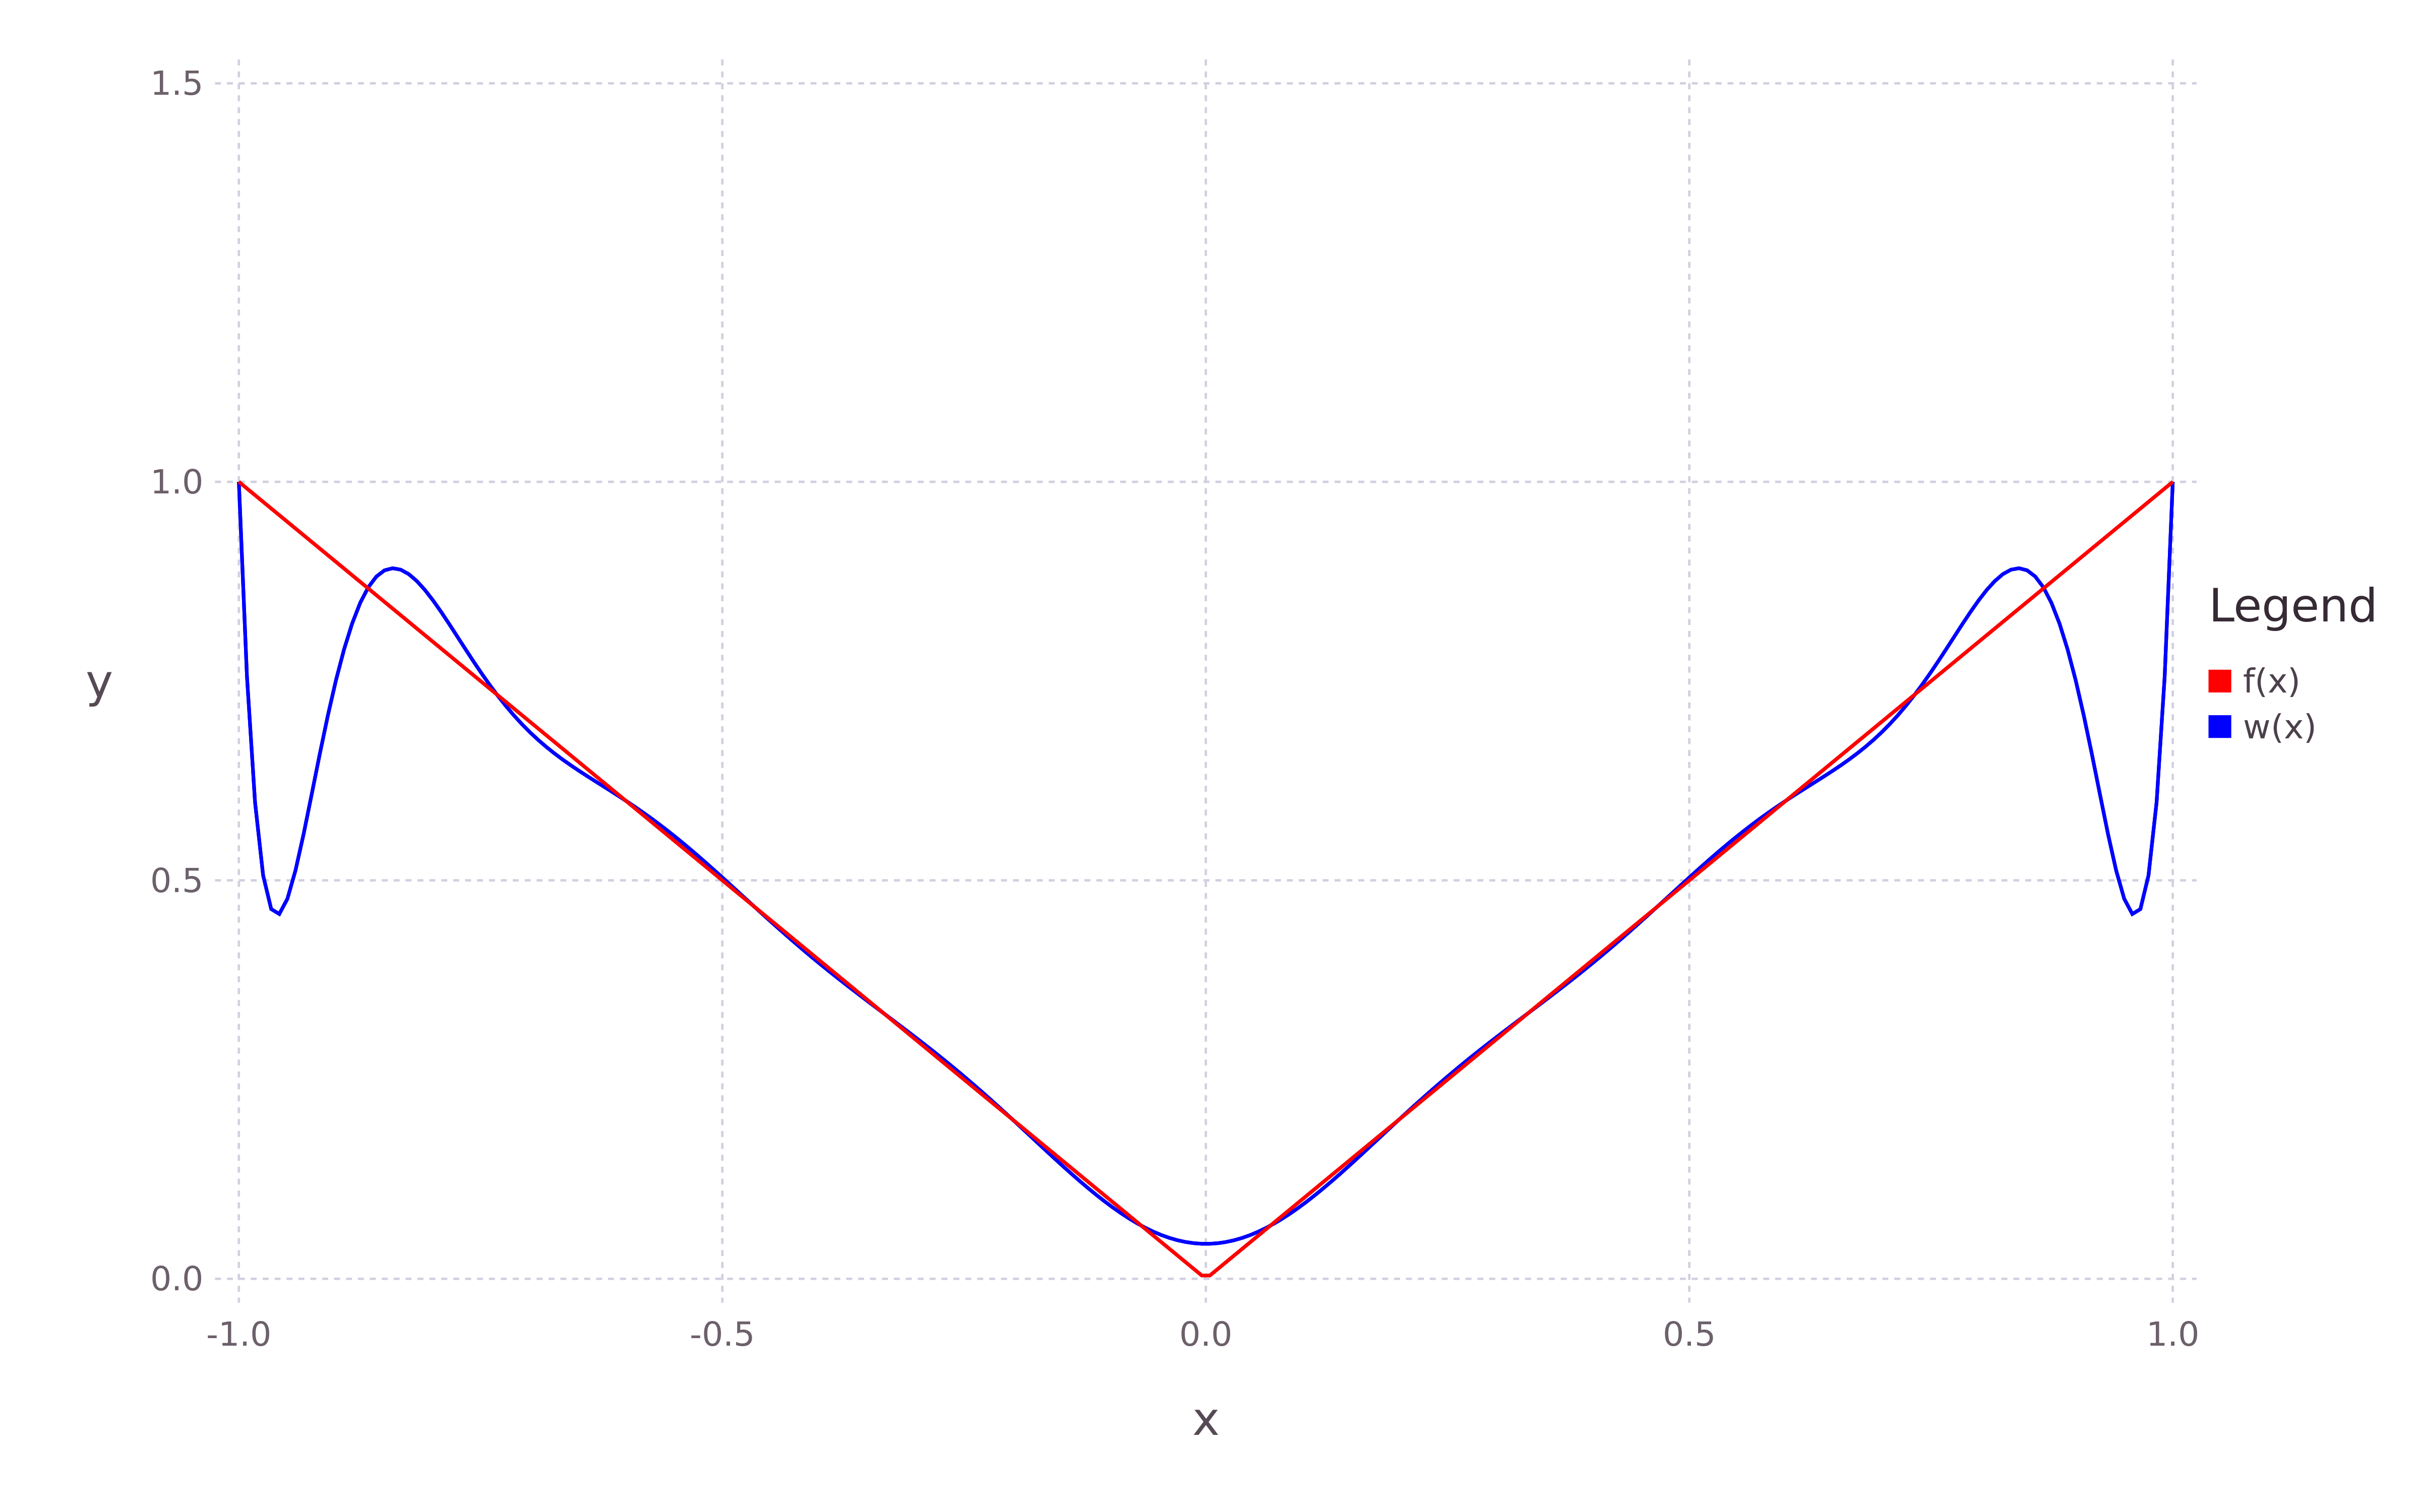
\includegraphics[width=0.5\textwidth]{zad6/plota3.png}}
  			\caption{Wykres funkcji $|x|$ oraz jej wielomianu interpolacyjnego o zadanym stopniu.}
  			\label{fig:3}
		\end{figure}		
	
		
		\begin{figure}[!h]
			\centering
			\subfloat[1.][$n=5$]{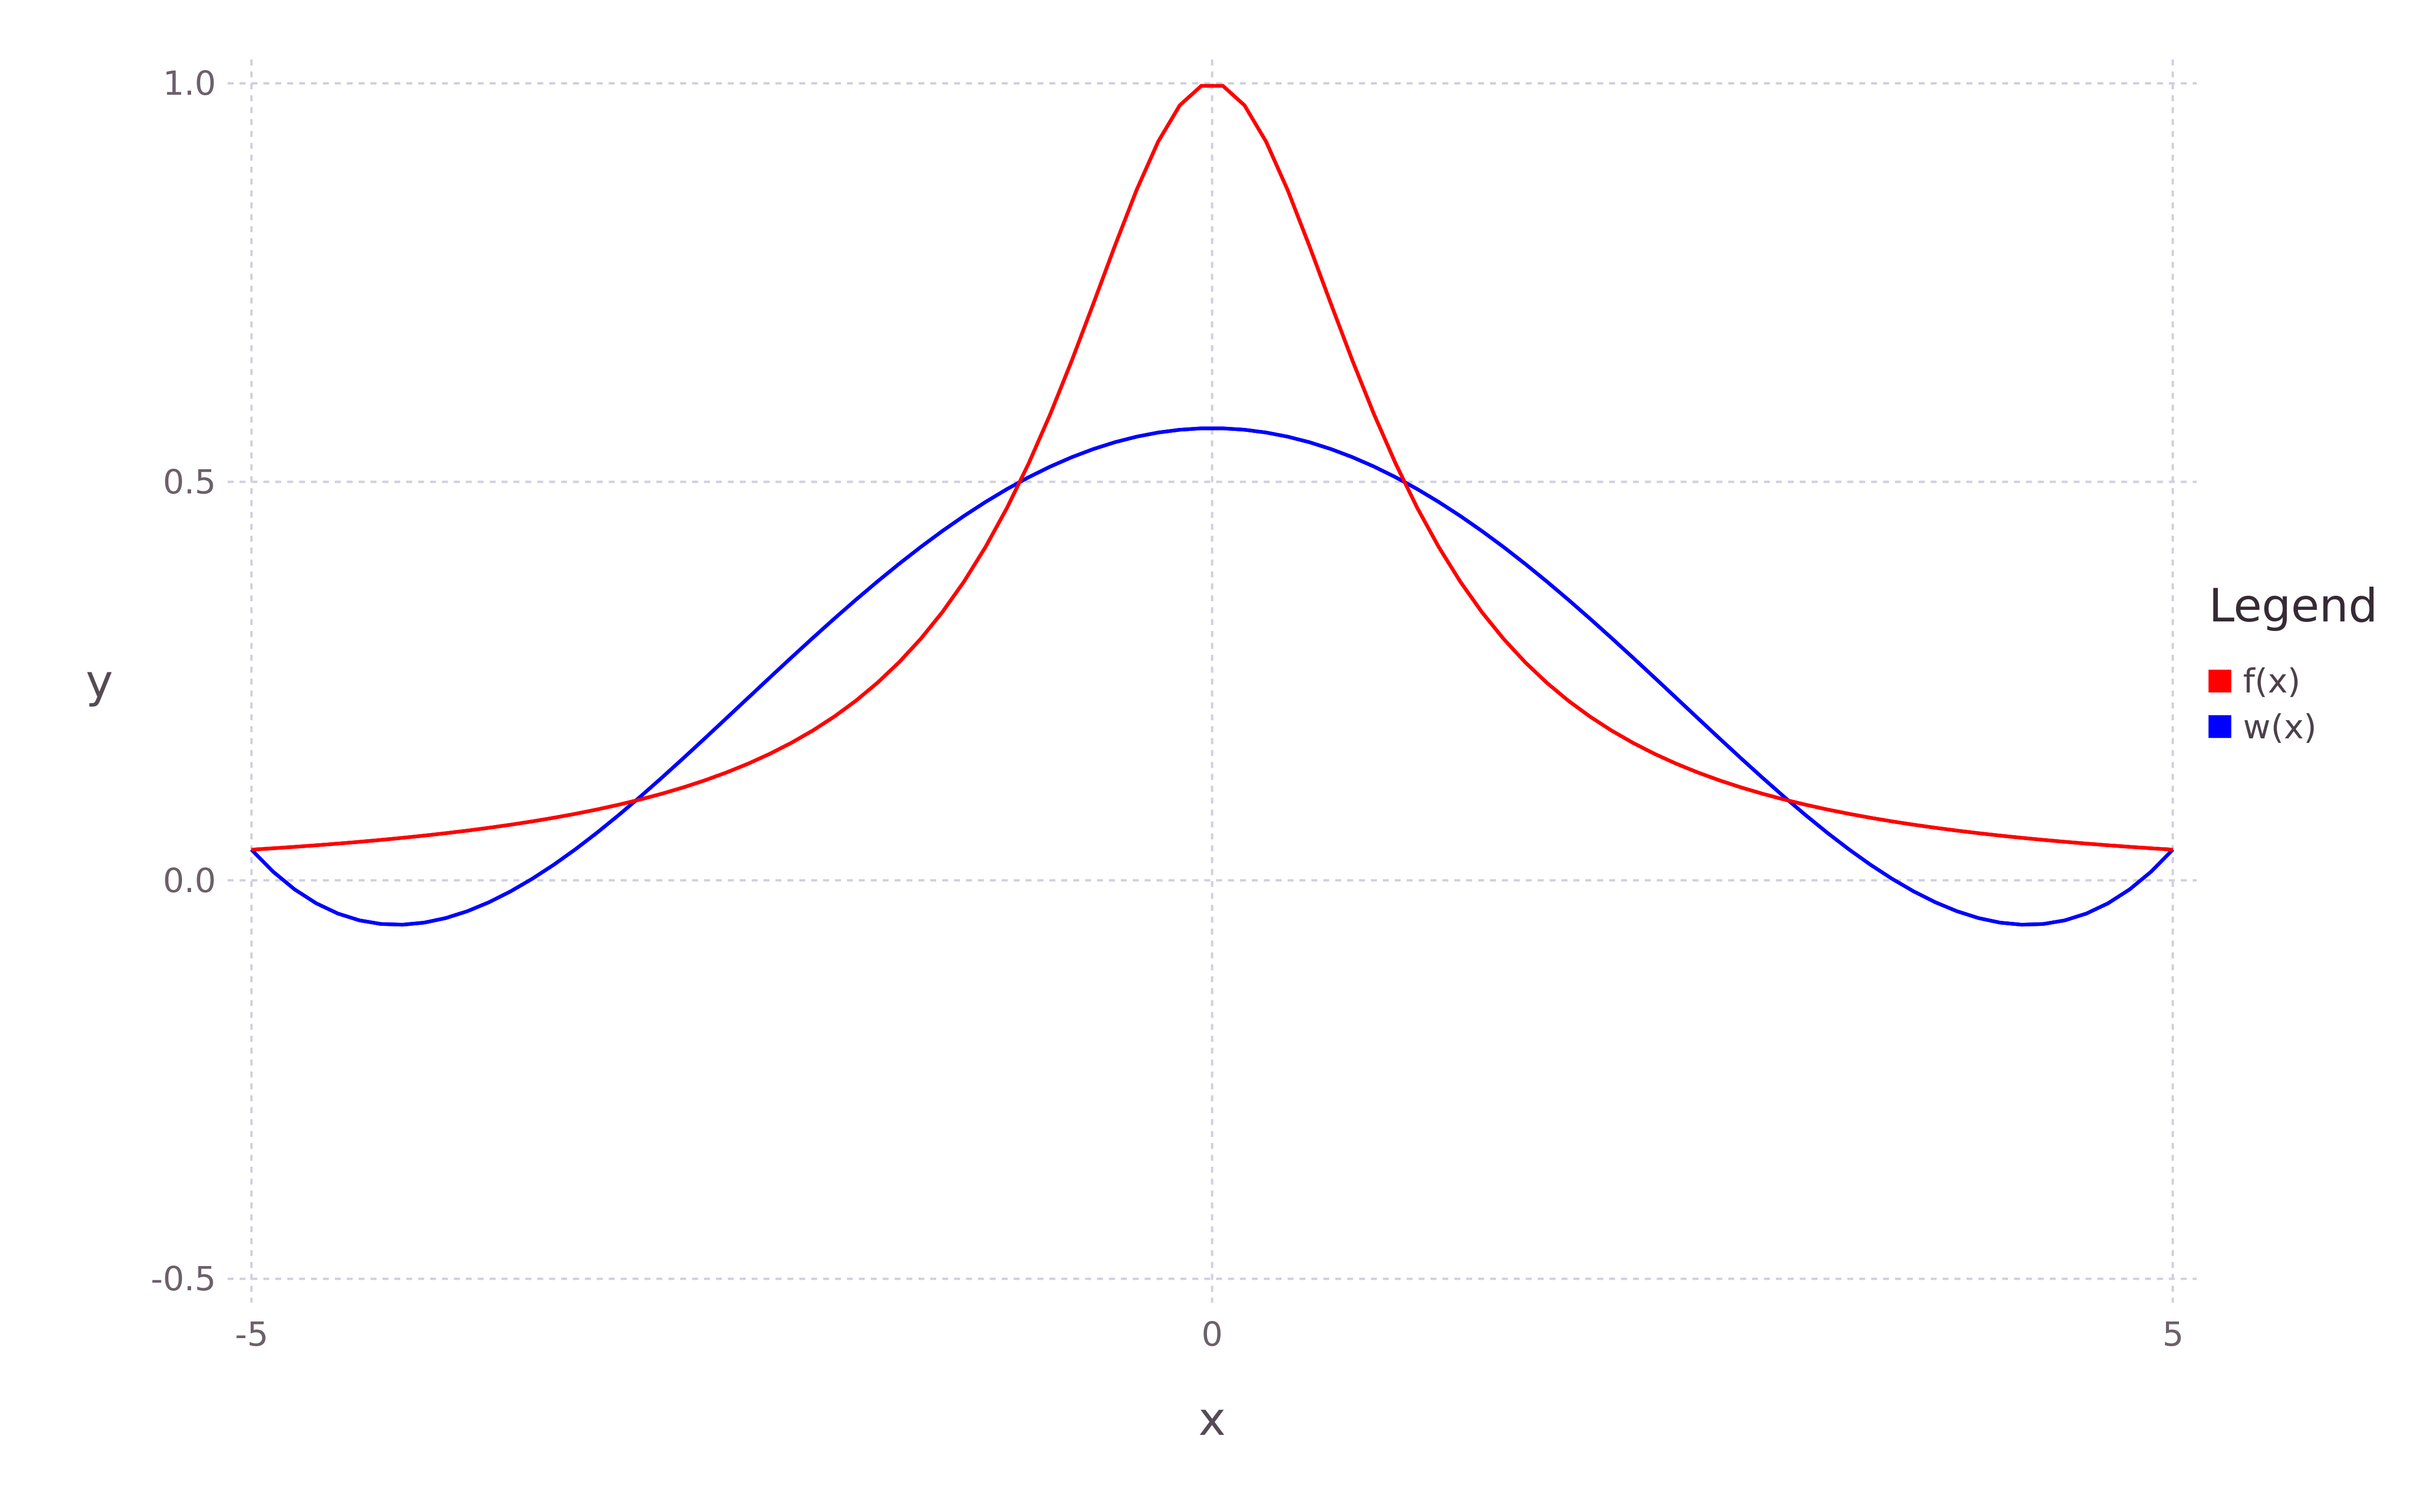
\includegraphics[width=0.5\textwidth]{zad6/plotb1.png}} \hfill
			\subfloat[2.][$n=10$]{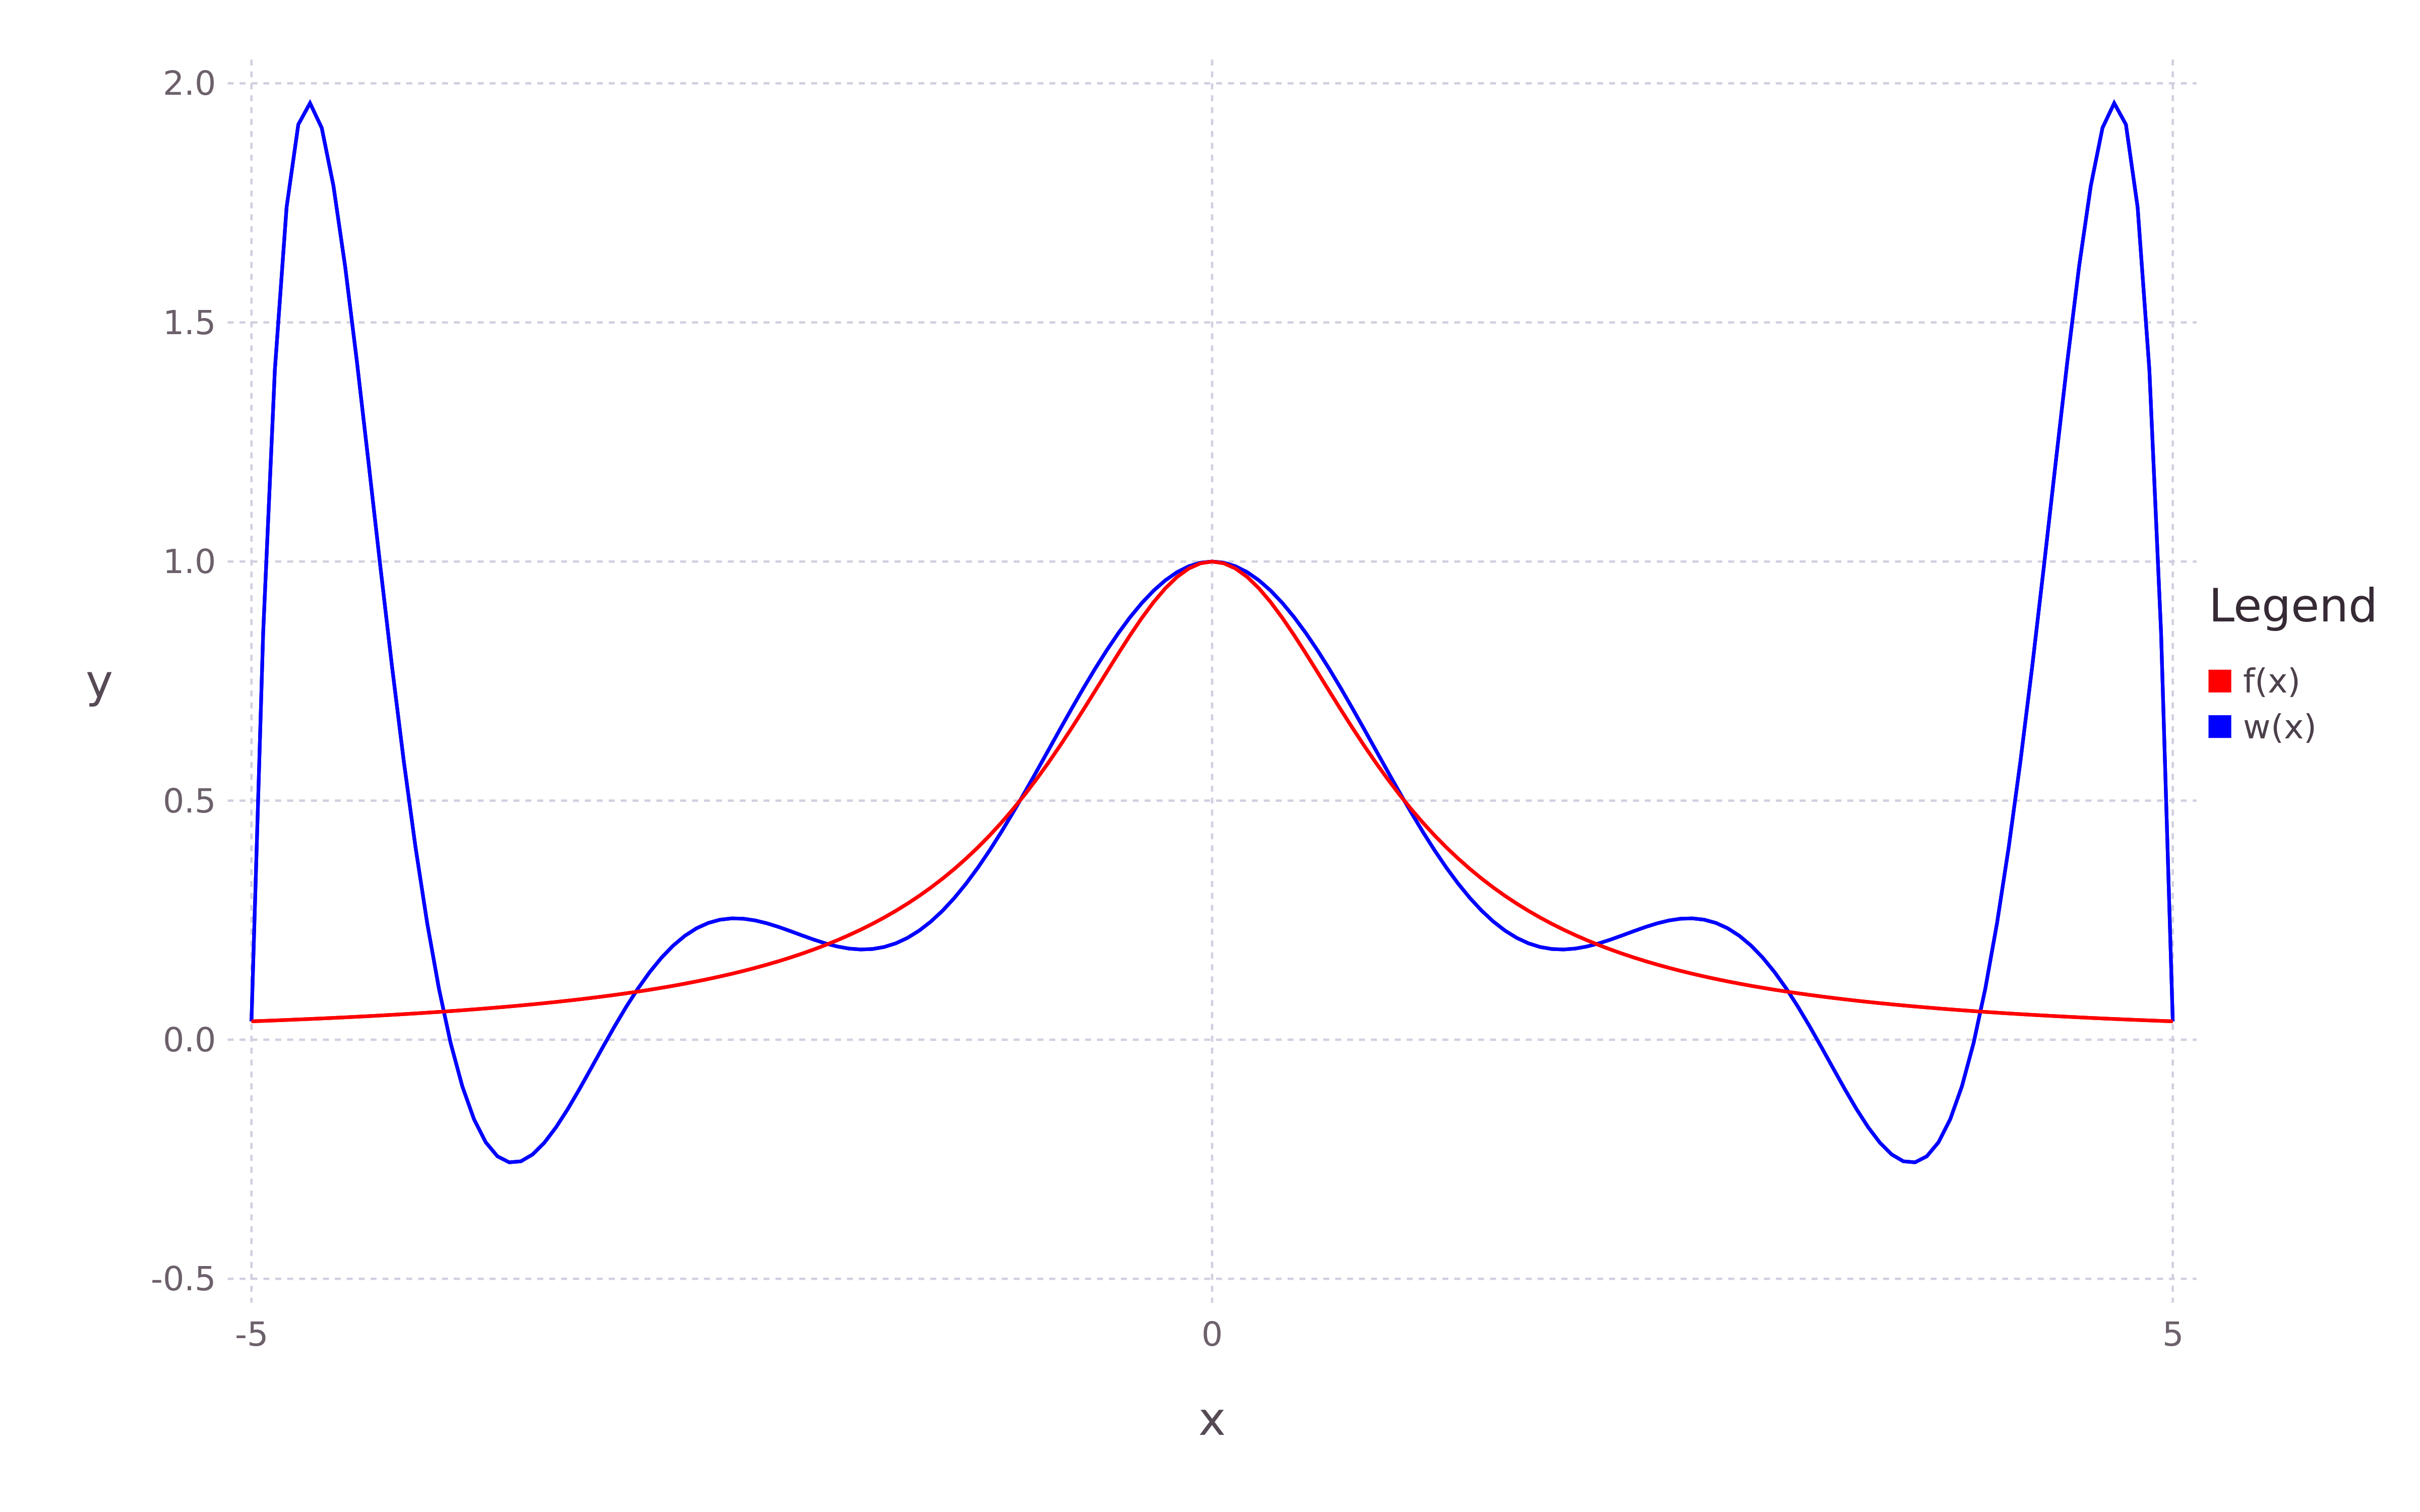
\includegraphics[width=0.5\textwidth]{zad6/plotb2.png}} \hfill
			\subfloat[3.][$n=15$]{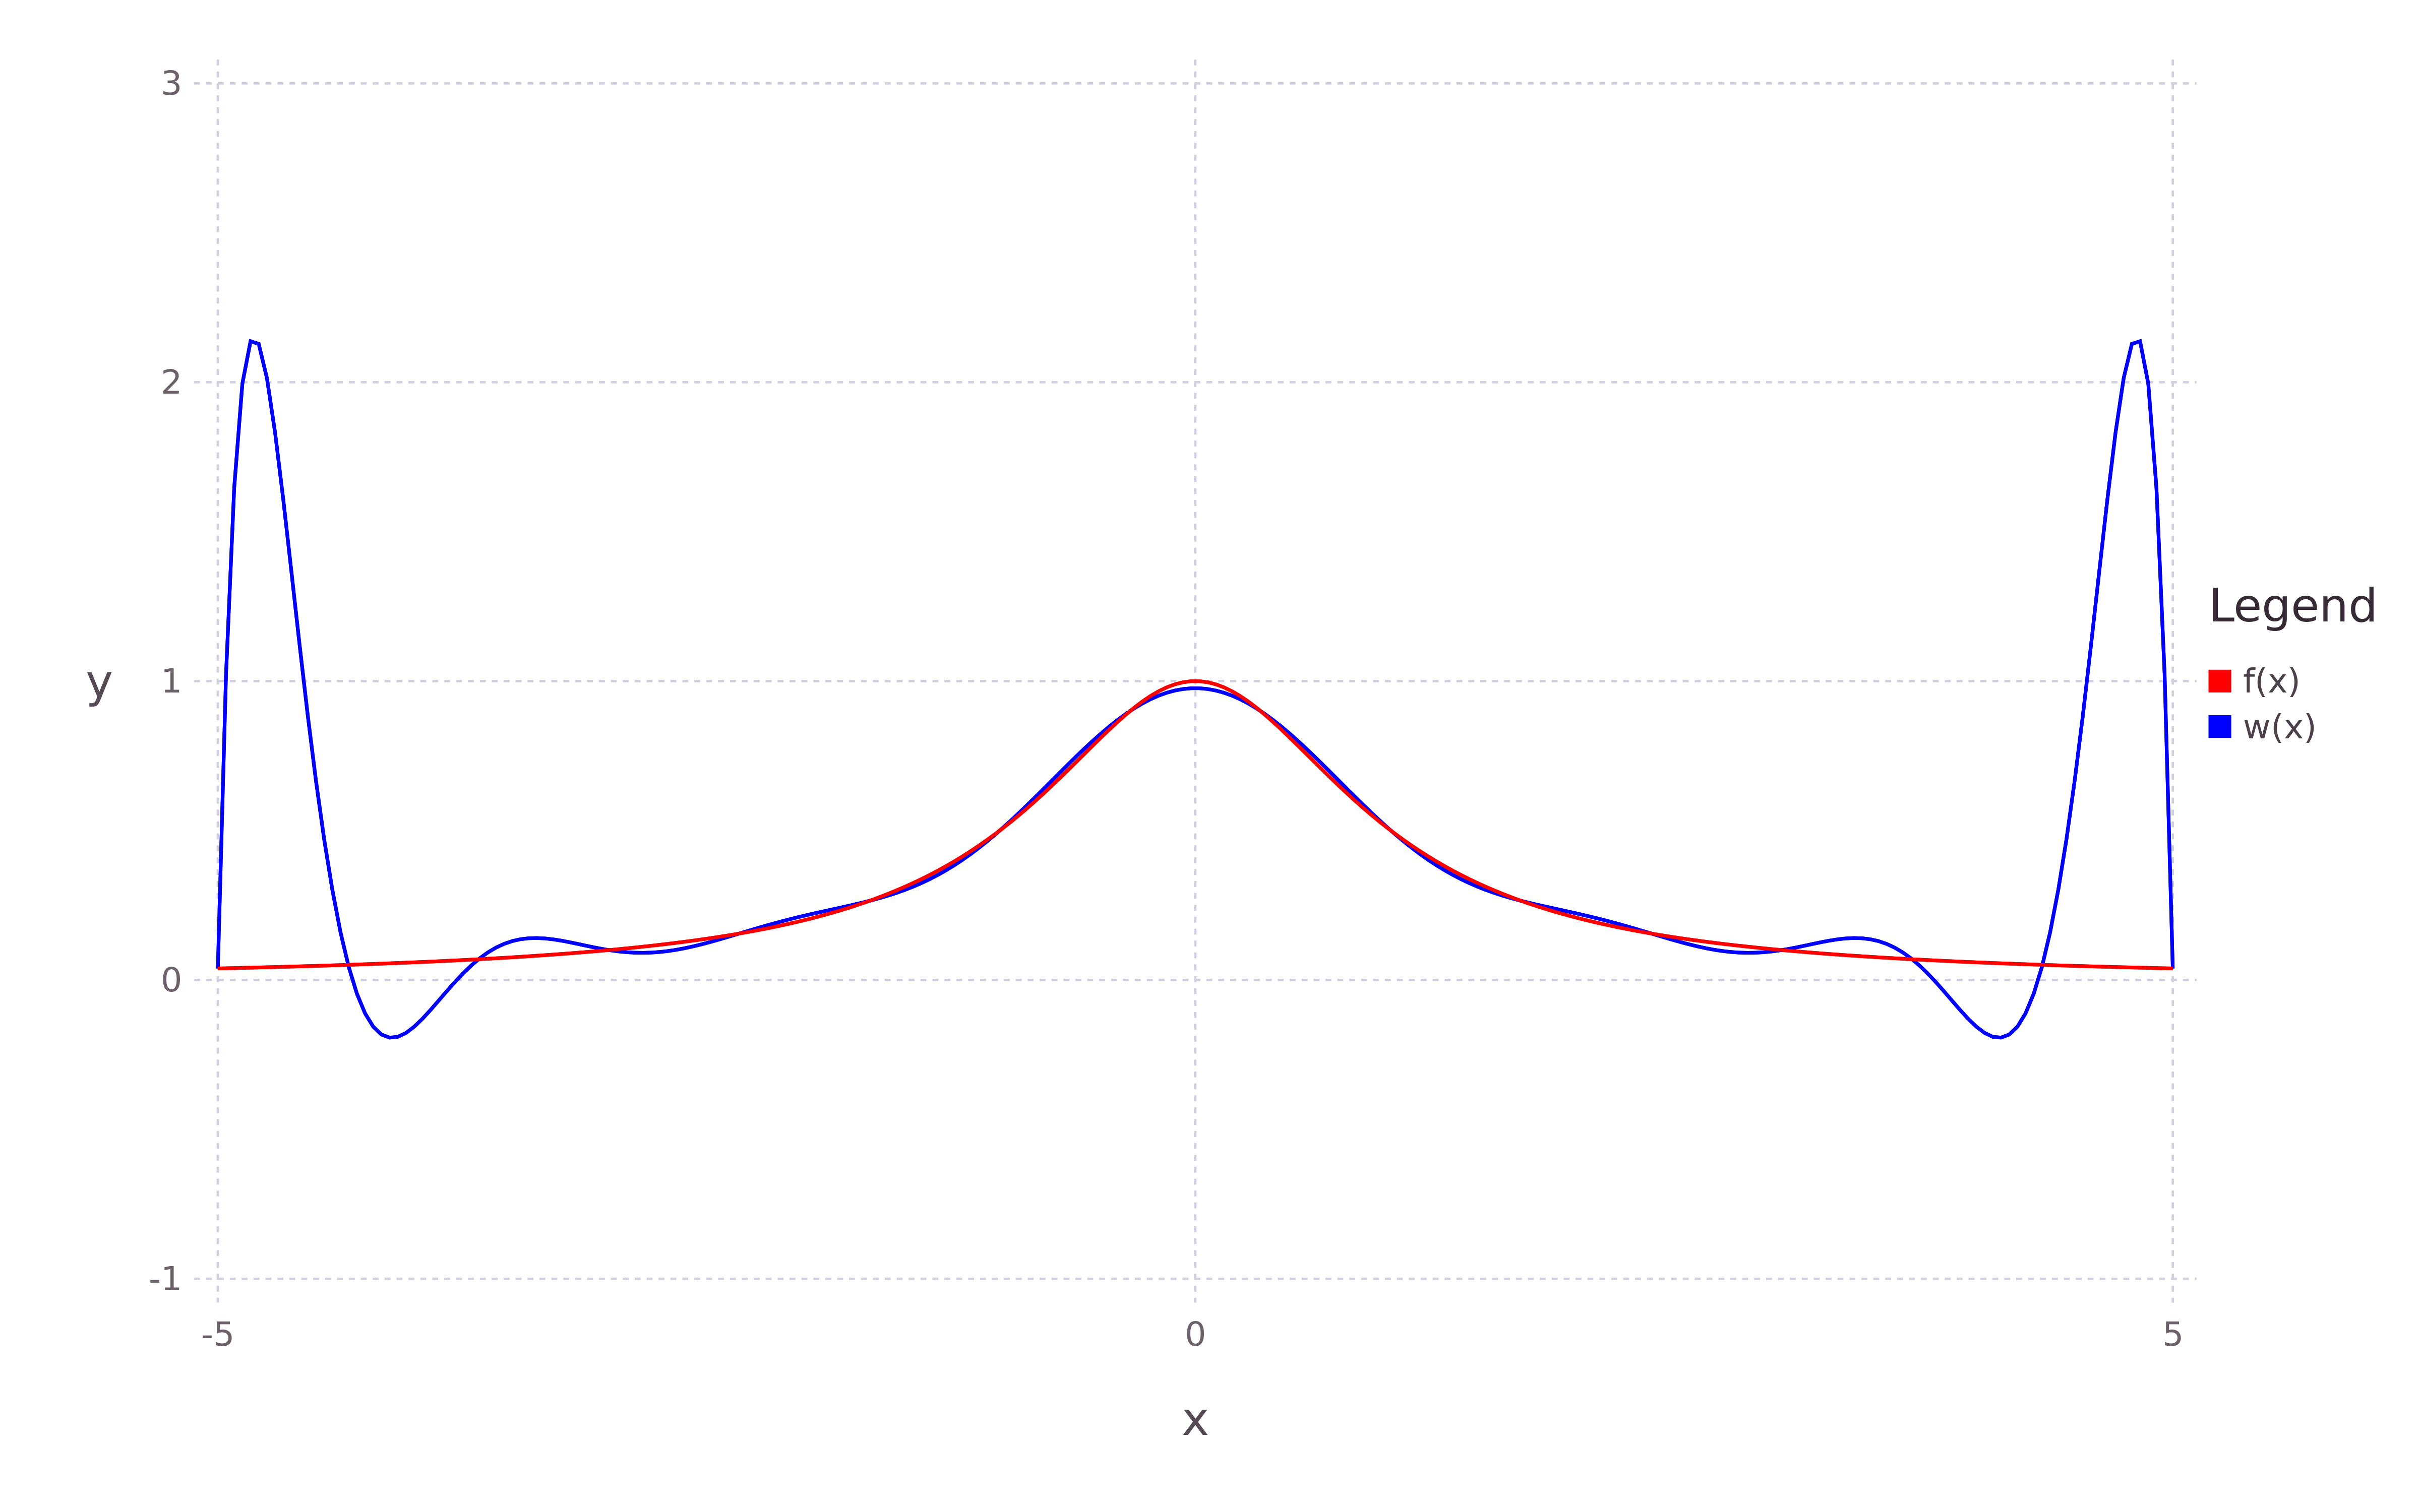
\includegraphics[width=0.5\textwidth]{zad6/plotb3.png}}
  			\caption{Wykres funkcji $\frac{1}{1+x^2}$ oraz jej wielomianu interpolacyjnego o zadanym stopniu.}
  			\label{fig:4}
		\end{figure}	
	\subsection{Wnioski}	
		Wyniki uzyskane dla tego zadania pokazują wyraźne rozbieżności pomiędzy wykresem funkcji a jej wielomianami interpolacyjnymi.
		W przypadku $|x|$ duże odchylenia spowodowane były głównie faktem, iż nie jest ona różniczkowalna.
		
		Dla drugiej funkcji zaobserwować można ciekawe zjawisko. Otóż początkowo ze wzrostem liczby węzłów przybliżenie poprawia się, jednak sytuacja ulega zmianie wraz z dalszym zwiększaniem $n$ --- widoczne jest znaczne odchylenie, szczególnie uwydatnione na końcach przedziałów. Taki efekt nosi nazwę zjawiska Rungego i oznacza pogorszenie jakości interpolacji wielomianowej, mimo zwiększenia liczby jej węzłów.
		Zastosowanie podziału równoległego skutkuje stosunkowo niewielką liczbą punktów na krawędziach przedziału, przez co wielomian interpolacyjny zdecydowanie odbiega tam od właściwej wartości funkcji, zaś stan ten pogarsza się przy zagęszczeniu węzłów równoodległych.
		Aby zwiększyć dokładność interpolacji należy zatem zmienić rozkład punktów. Taki problem sformułował rosyjski matematyk P.L. Czebyszew, jako problem znalezienia wielomianu, który najlepiej przybliżałby zero na danym przedziale. 
		
		W celu uniknięcia zaobserwowanych błędów najlepszym rozwiązaniem byłoby zastosowanie interpolacji z węzłami rozmieszczonymi gęściej w pobliżu miejsc "oscylacji" (np. miejsca zerowe wielomianu Czebyszewa).
		

\end{document}